\documentclass[12pt,twoside]{article}
\usepackage{weiiszablonzmodyfikowany}

% Imię i nazwisko autora projektu
\author{Hubert Lech}

% Numer indeksu autora (np. 123456)
\studentID{177827 2EF-DI P09}

% Tytuł pracy (należy podać pełny tytul pracy)
\title{Sztuczna Inteligencja\\Projekt\\[0.4em]\large  Klasyfikacja głosowań kongresowych\\ z wykorzystaniem sieci neuronowej uczonej algorytmem wstecznej propagacji błędu z przyśpieszeniem metodą momentum (MLP\_M)}

% Prowadzący
\supervisor{dr hab. inż. prof. PRz Roman Zajdel}

\begin{document}

% strona tytułowa
\maketitle

\blankpage

% spis treści
\tableofcontents

\section{Cel projektu}

Celem projektu jest realizacja sieci neuronowej do klasyfikacji głosowań kongresowych. Głównym wyzwaniem badawczym jest przewidzenie przynależności partyjnej kongresmena (demokrata czy republikanin) na podstawie jego głosowań w 16 kluczowych kwestiach w 1984 roku. Dodatkowym zadaniem jest zbadanie wpływu różnych parametrów sieci na skuteczność klasyfikacji. Projekt ma na celu nie tylko osiągnięcie wysokiej dokładności klasyfikacji, ale także zrozumienie, które cechy głosowań są najbardziej istotne dla rozróżnienia między partiami politycznymi. Sieć zrealizowana została w języku Python.

\section{Dane}
\subsection{Zestaw danych}

Zestaw danych użyty w projekcie (Congressional Voting Records) pochodzi z UCI Machine Learning Repository i zawiera informacje o głosowaniach kongresmenów w 1984 roku \cite{uciVoting}. Każdy rekord reprezentuje jednego kongresmena i zawiera 16 atrybutów odpowiadających jego głosowaniom w kluczowych kwestiach, a także etykietę klasy (demokrata lub republikanin). Wartości atrybutów są kodowane symbolicznie: \texttt{y} oznacza tak, \texttt{n} oznacza nie oraz \texttt{?}. W tym zbiorze \texttt{?} nie oznacza klasycznego braku danych, lecz głos inny niż \texttt{y}/\texttt{n} (np. \emph{present} lub brak jednoznacznie zadeklarowanego stanowiska).

Zestaw zawiera 435 rekordów, z czego 61,4\% (267) należy do klasy demokratów, a 38,6\% (168) do republikanów. Każdy rekord składa się z 17 atrybutów: 16 atrybutów głosowań oraz 1 atrybutu klasy.

\begin{figure}[h!]
\centering

\includegraphics[width=0.65\textwidth]{\detokenize{wykresy/rozklad_klas.png}}
\caption{Rozkład klas w zbiorze danych}
\label{fig:rozklad_klas}
\end{figure}

Opis poszczególnych atrybutów głosowań jest następujący:
\begin{itemize}[label={\textbullet}]
\item \texttt{handicapped-infants} -- ustawa dotycząca ochrony i leczenia noworodków z niepełnosprawnościami (tak/nie)
\item \texttt{water-project-cost-sharing} -- podział kosztów projektów wodnych między budżet federalny a lokalny (tak/nie)
\item \texttt{adoption-of-the-budget-resolution} -- głosowanie nad ogólnym planem budżetowym państwa na dany rok (tak/nie)
\item \texttt{physician-fee-freeze} -- zamrożenie stawek opłat pobieranych przez lekarzy w ramach programu Medicare (tak/nie)
\item \texttt{el-salvador-aid} -- przyznanie pomocy finansowej i wojskowej dla rządu Salwadoru podczas wojny domowej (tak/nie)
\item \texttt{religious-groups-in-schools} -- możliwość organizowania spotkań grup religijnych w publicznych szkołach średnich (tak/nie)
\item \texttt{anti-satellite-test-ban} -- zakaz testowania broni antysatelitarnej przez USA (tak/nie)
\item \texttt{aid-to-nicaraguan-contras} -- wsparcie finansowe dla rebeliantów walczących z rządem w Nikaragui (tak/nie)
\item \texttt{mx-missile} -- finansowanie produkcji i rozmieszczenia międzykontynentalnych pocisków (tak/nie)
\item \texttt{immigration} -- reforma prawa imigracyjnego (tak/nie)
\item \texttt{synfuels-corporation-cutback} -- ograniczenie funduszy dla korporacji zajmującej się paliwami syntetycznymi (tak/nie)
\item \texttt{education-spending} -- zwiększenie federalnych nakładów finansowych na edukację publiczną (tak/nie)
\item \texttt{superfund-right-to-sue} -- kwestie dotyczące funduszu Superfund (oczyszczanie toksycznych odpadów) i prawa obywateli do pozywania zanieczyszczających (tak/nie)
\item \texttt{crime} -- rozwiązania wynikające z kompleksowej ustawy o zwalczaniu przestępczości (tak/nie)
\item \texttt{duty-free-exports} -- przepisy dotyczące eksportu bezcłowego i preferencji handlowych (tak/nie)
\item \texttt{export-administration-act-south-africa} -- ograniczenia handlowe i sankcje wobec RPA w odpowiedzi na politykę apartheidu (tak/nie)
\end{itemize}

\subsection{Brakujące dane}
W zbiorze dane oznaczone symbolem \texttt{?} występują w 248 rekordach, co stanowi 57\% wszystkich rekordów. Jest to znacząca ilość, która nie może zostać zignorowana i usunięta, dlatego w etapie przygotowania danych kodowane są jako neutralne 0. Taki sposób kodowania pozwala na zachowanie informacji, jednocześnie umożliwiając modelowi uczenie się na podstawie tych danych.

Przykładowe rekordy ze zbioru wejściowego przedstawiono na listingu \ref{lst:house_votes_missing}.

\begin{samepage}
\begin{center}
\begin{minipage}{\linewidth}

\lstinputlisting[
inputencoding=utf8/cp1250,
firstline=1,
lastline=12,
breaklines=true,
numbers=left,
frame=single,
caption={Przyk{\l}adowe rekordy ze zbioru wej\'sciowego z brakuj\k{a}cymi danymi},
label={lst:house_votes_missing}
] {house-votes-84.data}

\end{minipage}
\end{center}
\end{samepage}

\subsection{Przygotowanie danych}
W ramach przygotowania danych zastosowano stały schemat, w którym głosy na tak (y) zamieniono na wartość 1, głosy przeciwne (n) na -1, natomiast wszelkie braki, wstrzymania się lub nieobecności oznaczone jako ? zamieniono na neutralną wartość 0.

Równocześnie przekształcono etykietę klasy, przypisując demokratom identyfikator -1, a republikanom 1. Cała operacja została zrealizowana przy użyciu biblioteki Pandas, co pozwoliło na szybkie przetworzenie rekordów do postaci czystego pliku CSV.

Implementację transformacji danych przedstawiono na listingu \ref{lst:transformacja_py}.



\lstinputlisting[
language=Python,
inputencoding=utf8/cp1250,
firstline=1,
lastline=80,
breaklines=true,
numbers=left,
frame=single,
caption={Skrypt przygotowania danych do formatu \texttt{CSV}},
label={lst:transformacja_py}
] {transformacja.py}


Przykładowe rekordy po transformacji przedstawiono na listingu \ref{lst:transformed_votes_sample}.


\lstinputlisting[
inputencoding=utf8/cp1250,
firstline=1,
lastline=12,
breaklines=true,
numbers=left,
frame=single,
caption={Przyk{\l}adowe rekordy po transformacji},
label={lst:transformed_votes_sample}
] {transformed_votes.csv}


Na końcu etapu przygotowania danych wykonano dodatkową konwersję pliku \texttt{CSV} do formatu \texttt{Hickle} przy pomocy skryptu \ref{lst:hkl_py}. Celem tej operacji było przyspieszenie i uproszczenie dalszego wczytywania danych w programie uczącym: zamiast każdorazowo parsować plik tekstowy \texttt{CSV}, aplikacja ładuje bezpośrednio gotowe tablice \texttt{NumPy} z pliku binarnego.


\lstinputlisting[
language=Python,
inputencoding=utf8/cp1250,
firstline=1,
lastline=40,
breaklines=true,
numbers=left,
frame=single,
caption={Skrypt konwersji z formatu \texttt{CSV} do \texttt{Hickle} \texttt{.hkl}},
label={lst:hkl_py}
]{hkl.py}


Skrypt zapisuje dane w postaci listy: \texttt{[x, y\_t, x\_norm, x\_n\_s, y\_t\_s]}. W tym projekcie przyjęto \texttt{x\_norm = x}, a część oznaczona jako zbiór testowy w pliku \texttt{.hkl} jest taka sama jak zbiór pełny (\texttt{x\_n\_s = x\_norm}, \texttt{y\_t\_s = y\_t}). Nie wykonano tu stałego podziału typu train/test, ponieważ właściwy podział realizowany jest później dynamicznie w trakcie walidacji krzyżowej \texttt{StratifiedKFold}.

\subsection{Wizualizacja danych}
W celu lepszego zrozumienia rozkładu głosowań w zbiorze danych, przeprowadzono wizualizację procentowego udziału głosów wewnątrz każdej partii dla poszczególnych kwestii. Wykresy te pozwalają na szybkie zidentyfikowanie, które kwestie były bardziej kontrowersyjne i jak różniły się stanowiska demokratów i republikanów.

\begin{figure}[h!]
\centering

\includegraphics[width=0.9\textwidth]{\detokenize{wykresy/dzieci_z_niepełnosprawnością.png}}
\caption{Rozkład głosów dla kwestii: dzieci z niepełnosprawnością}
\label{fig:viz_handicapped_infants}
\end{figure}

\begin{figure}[h!]
\centering

\includegraphics[width=0.9\textwidth]{\detokenize{wykresy/koszty_projektów_wodnych.png}}
\caption{Rozkład głosów dla kwestii: koszty projektów wodnych}
\label{fig:viz_water_project_costs}
\end{figure}

\begin{figure}[h!]
\centering

\includegraphics[width=0.9\textwidth]{\detokenize{wykresy/rezolucja_budżetowa.png}}
\caption{Rozkład głosów dla kwestii: rezolucja budżetowa}
\label{fig:viz_budget_resolution}
\end{figure}

\begin{figure}[h!]
\centering

\includegraphics[width=0.9\textwidth]{\detokenize{wykresy/zamrożenie_opłat_lekarzy.png}}
\caption{Rozkład głosów dla kwestii: zamrożenie opłat lekarzy}
\label{fig:viz_physician_fee_freeze}
\end{figure}

\begin{figure}[h!]
\centering

\includegraphics[width=0.9\textwidth]{\detokenize{wykresy/pomoc_dla_salwadoru.png}}
\caption{Rozkład głosów dla kwestii: pomoc dla Salwadoru}
\label{fig:viz_el_salvador_aid}
\end{figure}

\begin{figure}[h!]
\centering

\includegraphics[width=0.9\textwidth]{\detokenize{wykresy/religia_w_szkołach.png}}
\caption{Rozkład głosów dla kwestii: religia w szkołach}
\label{fig:viz_religion_in_schools}
\end{figure}

\begin{figure}[h!]
\centering

\includegraphics[width=0.9\textwidth]{\detokenize{wykresy/testy_antysatelitarne.png}}
\caption{Rozkład głosów dla kwestii: testy antysatelitarne}
\label{fig:viz_antisatellite_tests}
\end{figure}

\begin{figure}[h!]
\centering

\includegraphics[width=0.9\textwidth]{\detokenize{wykresy/pomoc_dla_contras.png}}
\caption{Rozkład głosów dla kwestii: pomoc dla Contras}
\label{fig:viz_contras_aid}
\end{figure}

\begin{figure}[h!]
\centering

\includegraphics[width=0.9\textwidth]{\detokenize{wykresy/pociski_mx.png}}
\caption{Rozkład głosów dla kwestii: pociski MX}
\label{fig:viz_mx_missile}
\end{figure}

\begin{figure}[h!]
\centering

\includegraphics[width=0.9\textwidth]{\detokenize{wykresy/imigracja.png}}
\caption{Rozkład głosów dla kwestii: imigracja}
\label{fig:viz_immigration}
\end{figure}

\begin{figure}[h!]
\centering

\includegraphics[width=0.9\textwidth]{\detokenize{wykresy/paliwa_syntetyczne.png}}
\caption{Rozkład głosów dla kwestii: paliwa syntetyczne}
\label{fig:viz_synfuels}
\end{figure}

\begin{figure}[h!]
\centering

\includegraphics[width=0.9\textwidth]{\detokenize{wykresy/wydatki_na_edukację.png}}
\caption{Rozkład głosów dla kwestii: wydatki na edukację}
\label{fig:viz_education_spending}
\end{figure}

\begin{figure}[h!]
\centering

\includegraphics[width=0.9\textwidth]{\detokenize{wykresy/prawo_do_pozwów_(superfund).png}}
\caption{Rozkład głosów dla kwestii: prawo do pozwów (Superfund)}
\label{fig:viz_superfund_right_to_sue}
\end{figure}

\begin{figure}[h!]
\centering

\includegraphics[width=0.9\textwidth]{\detokenize{wykresy/przestępczość.png}}
\caption{Rozkład głosów dla kwestii: przestępczość}
\label{fig:viz_crime}
\end{figure}

\begin{figure}[h!]
\centering

\includegraphics[width=0.9\textwidth]{\detokenize{wykresy/eksport_bezcłowy.png}}
\caption{Rozkład głosów dla kwestii: eksport bezcłowy}
\label{fig:viz_duty_free_exports}
\end{figure}

\begin{figure}[h!]
\centering

\includegraphics[width=0.9\textwidth]{\detokenize{wykresy/eksport_do_rpa.png}}
\caption{Rozkład głosów dla kwestii: eksport do RPA}
\label{fig:viz_export_south_africa}
\end{figure}


\section{Część teoretyczna}

\subsection{Model neuronu}

Początki formalnego opisu neuronu w kontekście obliczeń wiążą się z pracą Warrena S. McCullocha i Waltera Pittsa z 1943 roku. McCulloch z zawodu był neurofizjologiem, a Pitts matematykiem, co przełożyło się na próbę połączenia wiedzy o biologicznym neuronie z precyzyjnym zapisem matematycznym \cite{geronML}. W najprostszym ujęciu sztuczny neuron można traktować jako element przetwarzający sygnały wejściowe, który waży je, sumuje i na tej podstawie wytwarza sygnał wyjściowy.

Na rysunku \ref{fig:model_perceptron_rosenblatt} przedstawiono schemat neuronu (perceptronu) z wejściami $x_1,\dots,x_L$ oraz odpowiadającymi im wagami $w_1,\dots,w_L$. Wagi opisują wpływ danego sygnału wejściowego na wynik neuronu: dodatnie wzmacniają wkład wejścia, a ujemne go osłabiają. Dodatkowo uwzględnia się wyraz wolny (bias) $b$, który pozwala przesunąć punkt równowagi sumy ważonej. Sygnał wyjściowy neuronu uzyskuje się, stosując funkcję aktywacji do pobudzenia.

\begin{figure}[h!]
\centering
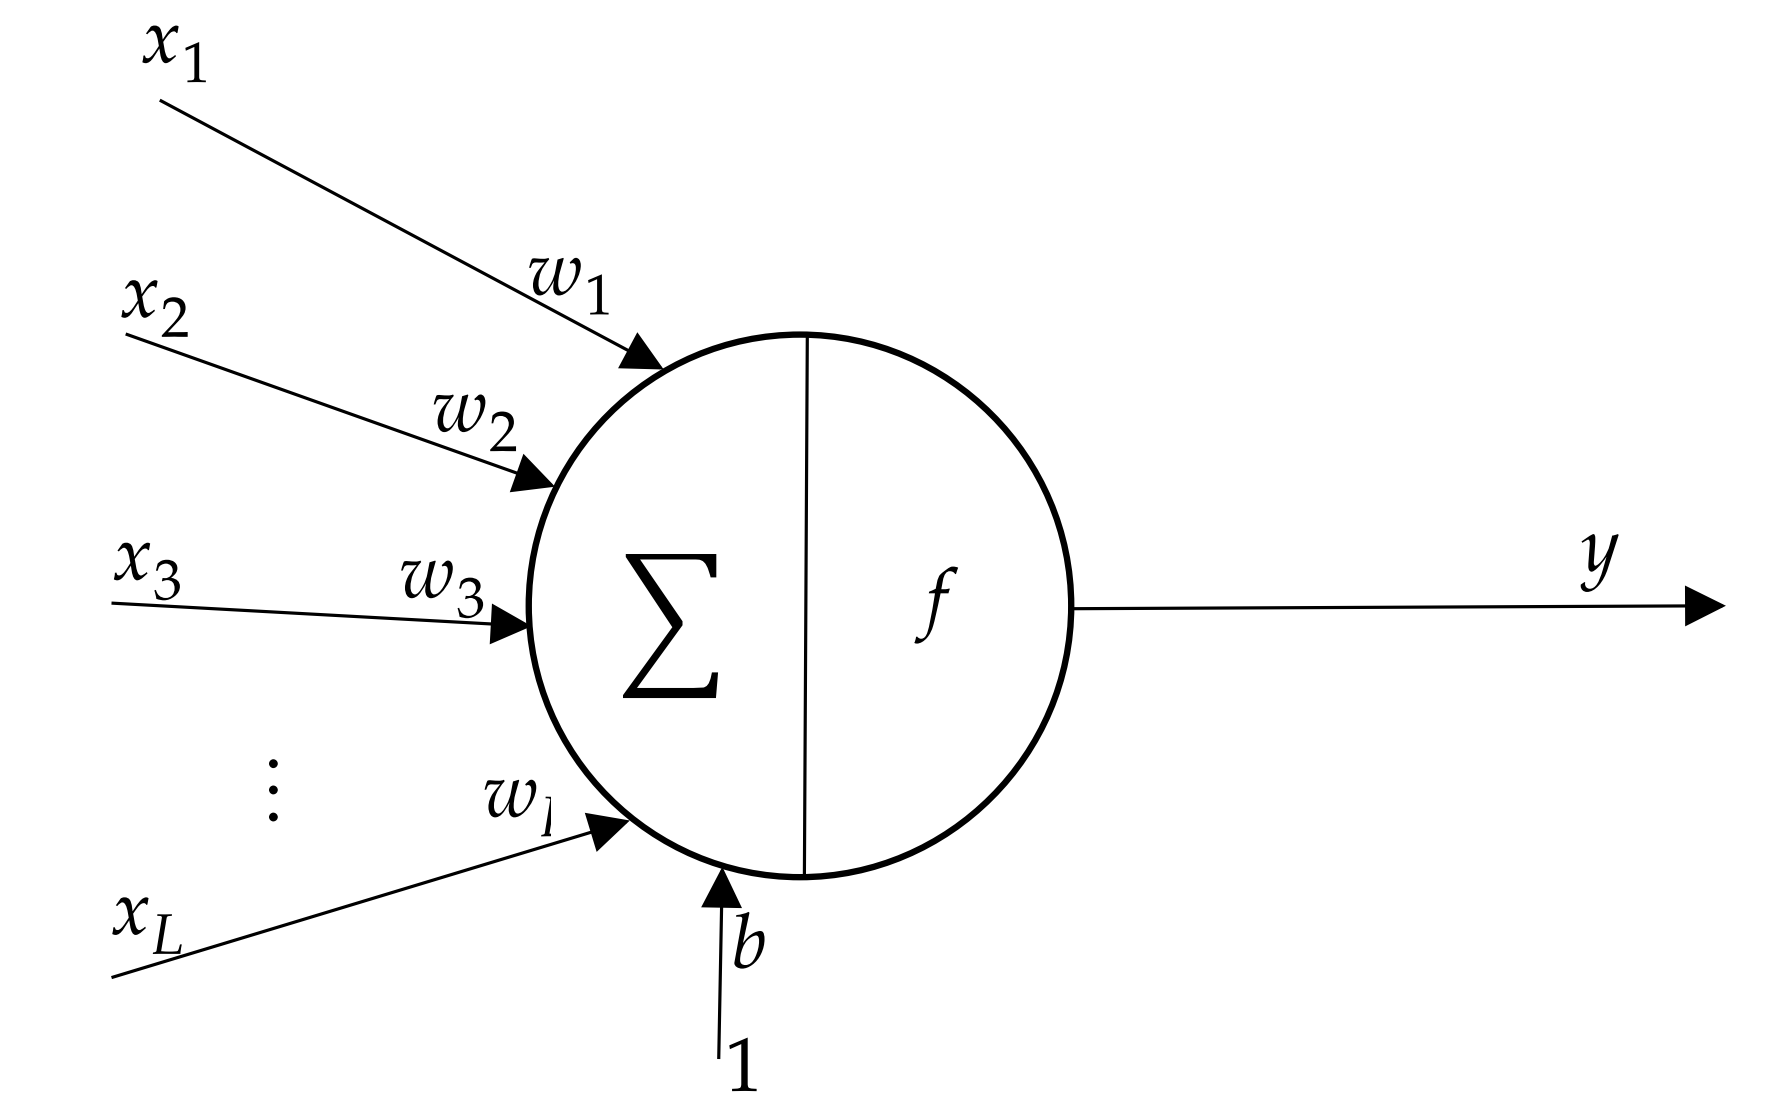
\includegraphics[width=0.8\textwidth]{figures/perceptron.png}
\caption{Schemat sztucznego neuronu \cite{zajdelLab}}
\label{fig:model_perceptron_rosenblatt}
\end{figure}

\subsection{Opis matematyczny sztucznego neuronu}

Pobudzenie neuronu można zapisać jako:
\begin{equation}
z = \sum_{j=1}^{L} w_j x_j + b.
\end{equation}

\subsubsection*{Gdzie:}
\begin{itemize}[label={\textbullet}]
\item $x_j$ -- $j$-ty sygnał wejściowy (atrybut)
\item $w_j$ -- waga odpowiadająca sygnałowi $x_j$
\item $b$ -- wyraz wolny (bias)
\item $z$ -- pobudzenie neuronu (suma ważona z biasem)
\item $L$ -- liczba sygnałów wejściowych
\end{itemize}
\subsection{Funkcja aktywacji}

W warstwach ukrytych zastosowano funkcję tangens hiperboliczny ($\tanh$):
\begin{equation}
h = \tanh(z).
\end{equation}

Dane wejściowe mają wartości z przedziału $\{-1,0,1\}$, czyli są centrowane wokół zera i nie wymagają dodatkowej normalizacji. To dobrze współgra z funkcją $\tanh$, która zwraca wartości z zakresu $(-1,1)$ i dobrze się sprawdza dla sygnałów symetrycznych względem zera.

\begin{figure}[h!]
\centering

\includegraphics[width=0.7\textwidth]{\detokenize{figures/tanh.png}}
\caption{Wykres funkcji aktywacji $\tanh$}
\label{fig:tanh_activation}
\end{figure}

W warstwie wyjściowej zastosowano funkcję $\tanh$:
\begin{equation}
y = \tanh(z).
\end{equation}

Taki wybór jest naturalny dla zadania binarnego, ponieważ etykiety klas mają postać $-1$ i $1$. Wyjście funkcji $\tanh$ można interpretować jako wynik dodatni lub ujemny, co bezpośrednio wspiera decyzję klasową przez znak wyjścia.



\subsection{Sieci jednokierunkowe jednowarstwowe}

W sieci jednowarstwowej neuronu ułożone są w jednej warstwie, a przepływ sygnału zachodzi od wejścia do wyjścia. Dla $L$ sygnałów wejściowych oraz $K$ neuronów wyjściowych można zapisać:
\begin{equation}
z_i = \sum_{j=1}^{L} w_{ij}x_j + b_i, \qquad i=1,\dots,K,
\end{equation}
\begin{equation}
y_i = f_i(z_i).
\end{equation}

W zapisie macierzowym:
\begin{equation}
\mathbf{z} = \mathbf{W}\mathbf{x} + \mathbf{b},
\end{equation}
\begin{equation}
\mathbf{y} = f(\mathbf{z}) = f(\mathbf{W}\mathbf{x}+\mathbf{b}).
\end{equation}

Uczenie pod nadzorem zakłada, że każdemu wektorowi wejściowemu $\mathbf{x}$ odpowiada pożądany wektor sygnałów wyjściowych $\hat{\mathbf{y}}$:
\begin{equation}
\mathbf{x} = [x_1,x_2,\dots,x_L]^T,
\qquad
\hat{\mathbf{y}} = [\hat{y}_1,\hat{y}_2,\dots,\hat{y}_K]^T.
\end{equation}
Para $\mathbf{x},\hat{\mathbf{y}}$ stanowi więc jedną próbkę uczącą, na podstawie której sieć koryguje swoje parametry. Jeżeli sieć nie jest jeszcze nauczona, jej odpowiedź $\mathbf{y}$ różni się od wartości oczekiwanej $\hat{\mathbf{y}}$, co prowadzi do powstania błędu:
\begin{equation}
\mathbf{e} = \hat{\mathbf{y}} - \mathbf{y}.
\end{equation}

Zadaniem procesu uczenia jest takie modyfikowanie wag i biasów, aby odpowiedź sieci $\mathbf{y}$ możliwie dobrze pokrywała się z odpowiedzią wzorcową $\hat{\mathbf{y}}$. Najczęściej sprowadza się to do minimalizacji funkcji celu, którą w tym przypadku przyjmuje się jako sumaryczny błąd kwadratowy $SSE$:
\begin{equation}
E = SSE = \frac{1}{2}\sum_{i=1}^{K} e_i^2.
\end{equation}

W praktyce uczenie przebiega iteracyjnie. W kolejnych cyklach, często nazywanych epokami, wagi są korygowane tak, aby stopniowo zmniejszać wartość błędu. Dla pojedynczej $j$-tej wagi $i$-tego neuronu zmianę można zapisać jako zależność rekurencyjną:
\begin{equation}
 w_{ij}(t+1) = w_{ij}(t) + \Delta w_{ij}(t),
\end{equation}
gdzie $t$ oznacza numer cyklu uczenia. Sam przyrost wag wyznacza się metodą największego spadku, która prowadzi parametry w kierunku najszybszego zmniejszania błędu:
\begin{equation}
\Delta w_{ij} = -\eta \frac{\partial E}{\partial w_{ij}},
\end{equation}
gdzie $\eta>0$ jest współczynnikiem uczenia. Znak minus wynika z faktu, że gradient wskazuje kierunek najszybszego wzrostu funkcji celu, a w uczeniu dąży się do jej minimalizacji.

Uwzględniając zależność błędu od wagi poprzez sygnał wyjściowy i pobudzenie neuronu, pochodną można rozpisać regułą łańcuchową:
\begin{equation}
\frac{\partial E}{\partial w_{ij}} = \frac{\partial E}{\partial y_i}\frac{\partial y_i}{\partial z_i}\frac{\partial z_i}{\partial w_{ij}}.
\end{equation}

Korzystając z definicji błędu, otrzymujemy:
\begin{equation}
\frac{\partial E}{\partial y_i} = y_i - \hat{y}_i.
\end{equation}

Z zależności neuronu
\begin{equation}
z_i = \sum_{j=1}^{L} w_{ij}x_j + b_i
\end{equation}
wynika:
\begin{equation}
\frac{\partial z_i}{\partial w_{ij}} = x_j.
\end{equation}

Po podstawieniu dostajemy ogólną regułę uczenia dla pojedynczej wagi:
\begin{equation}
\Delta w_{ij} = \eta\left(\hat{y}_i - y_i\right) f_i'\!\left(z_i\right) x_j.
\end{equation}

Jeżeli funkcja aktywacji ma postać tangensa hiperbolicznego, czyli $y_i = \tanh(z_i)$, to jej pochodna wynosi $f_i'(z_i)=1-y_i^2$. Wtedy reguła uczenia przyjmuje postać:
\begin{equation}
\Delta w_{ij} = \eta\left(\hat{y}_i - y_i\right)\left(1-y_i^2\right)x_j.
\end{equation}

Analogicznie można wyznaczyć poprawkę dla biasu:
\begin{equation}
\Delta b_i = \eta\left(\hat{y}_i - y_i\right)f_i'\!\left(z_i\right).
\end{equation}

W ten sposób kolejne epoki uczenia prowadzą do stopniowego zmniejszania błędu i dopasowywania odpowiedzi sieci do sygnałów wzorcowych \cite{zajdelLab}.



\subsection{Sieci neuronowe jednokierunkowe wielowarstwowe}

W sieci jednokierunkowej wielowarstwowej każda warstwa ma własną macierz wag $\mathbf{W}^{(l)}$, wektor przesunięć $\mathbf{b}^{(l)}$, funkcję aktywacji $f^{(l)}(\cdot)$ oraz wektor wyjściowy $\mathbf{y}^{(l)}$. W analizowanym modelu występują dwie warstwy ukryte oraz jedna warstwa wyjściowa, oznaczone odpowiednio jako $1,2,3$. Propagacja sygnału przebiega więc od wejścia do wyjścia \cite{zajdelLab9}.

\begin{figure}[h!]
\centering
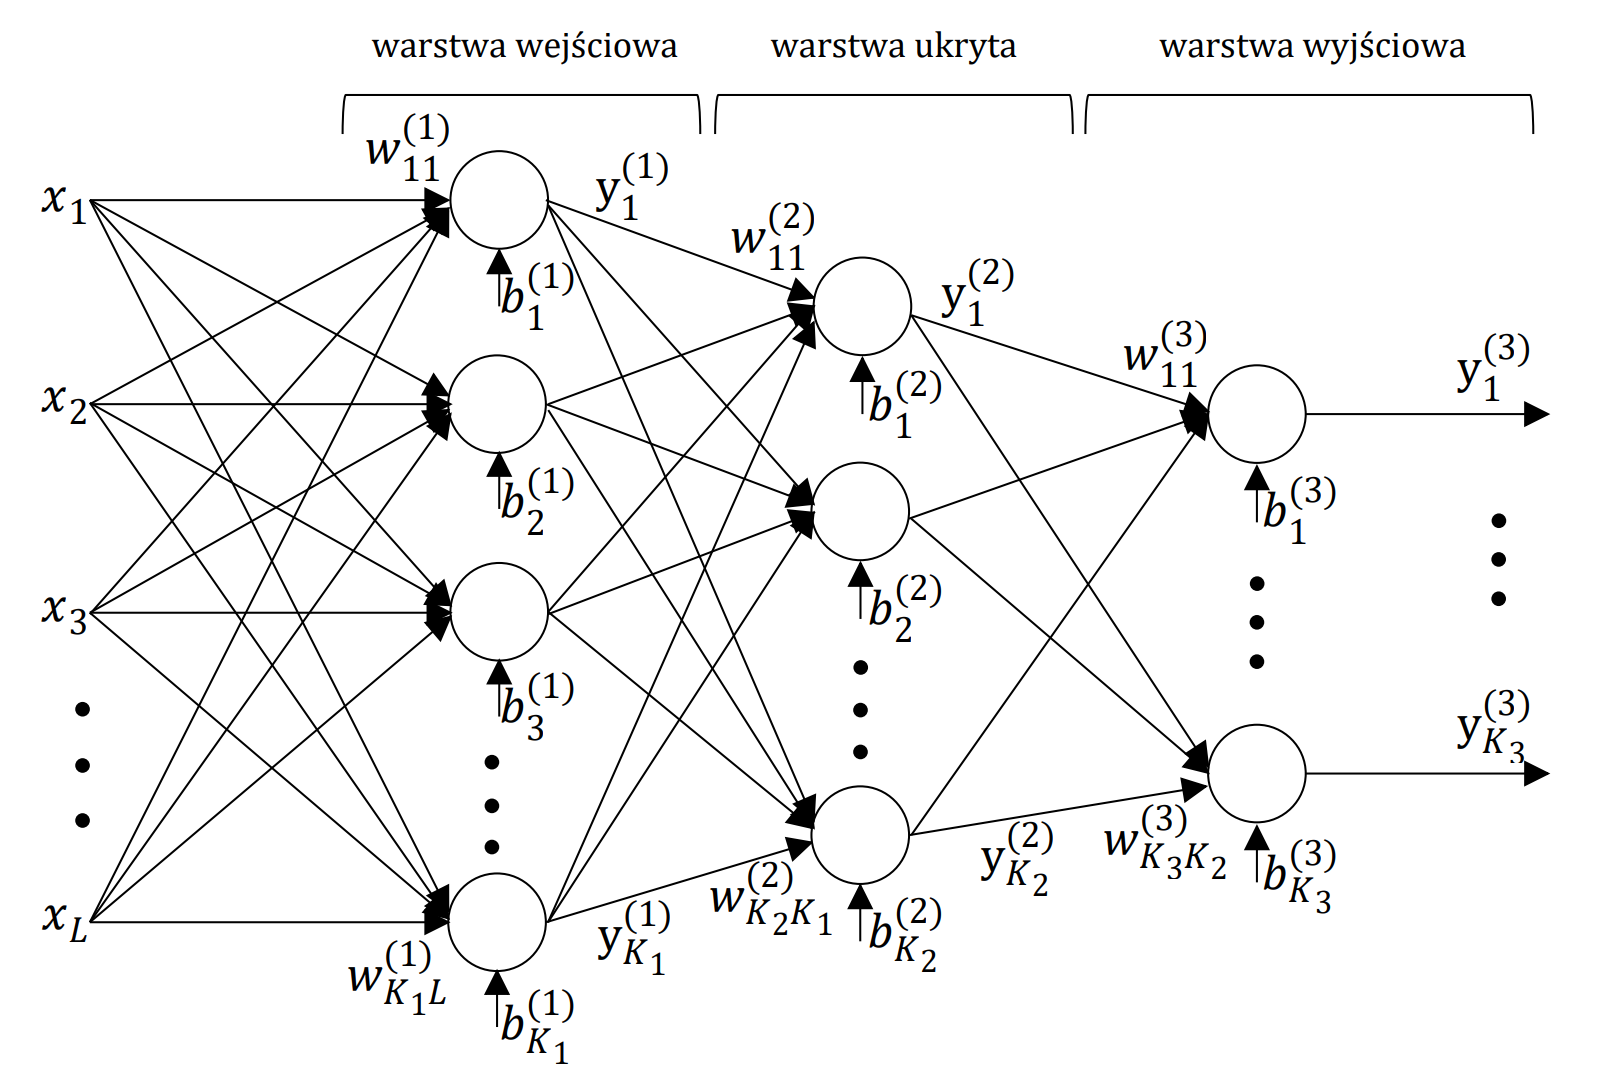
\includegraphics[width=0.9\textwidth]{figures/wielowarstwowa.png}
\caption{Schemat jednokierunkowej sieci wielowarstwowej \cite{zajdelLab9}}
\label{fig:mlp_arch}
\end{figure}

Dla wejścia $\mathbf{x}$ i kolejnych warstw otrzymujemy:
\begin{equation}
\mathbf{y}^{(1)} = f^{(1)}\!\left(\mathbf{W}^{(1)}\mathbf{x} + \mathbf{b}^{(1)}\right),
\end{equation}
\begin{equation}
\mathbf{y}^{(2)} = f^{(2)}\!\left(\mathbf{W}^{(2)}\mathbf{y}^{(1)} + \mathbf{b}^{(2)}\right),
\end{equation}
\begin{equation}
\mathbf{y}^{(3)} = f^{(3)}\!\left(\mathbf{W}^{(3)}\mathbf{y}^{(2)} + \mathbf{b}^{(3)}\right).
\end{equation}

Całą sieć można zapisać jako złożenie przekształceń:
\begin{equation}
\mathbf{y}^{(3)} = f^{(3)}\!\left(\mathbf{W}^{(3)} f^{(2)}\!\left(\mathbf{W}^{(2)} f^{(1)}\!\left(\mathbf{W}^{(1)}\mathbf{x}+\mathbf{b}^{(1)}\right)+\mathbf{b}^{(2)}\right)+\mathbf{b}^{(3)}\right).
\end{equation}

W notacji indeksowej dla neuronu $i_l$ warstwy $l$:
\begin{equation}
z_{i_l}^{(l)} = \sum_{i_{l-1}=1}^{K_{l-1}} w_{i_l i_{l-1}}^{(l)} y_{i_{l-1}}^{(l-1)} + b_{i_l}^{(l)},
\qquad
y_{i_l}^{(l)} = f^{(l)}\!\left(z_{i_l}^{(l)}\right),
\end{equation}
przy czym $\mathbf{y}^{(0)}=\mathbf{x}$ oraz dla pierwszej warstwy $K_0=L$.

\subsection{Algorytm wstecznej propagacji błędu}

Dla wyjścia trzeciej warstwy i sygnału zadanego $\hat{\mathbf{y}}^{(3)}$ funkcję błędu SSE zapisujemy jako:
\begin{equation}
E = SSE = \frac{1}{2}\sum_{i_3=1}^{K_3}\left(\hat{y}^{(3)}_{i_3}-y^{(3)}_{i_3}\right)^2.
\end{equation}

Po podstawieniu kolejnych warstw (łańcuchowo) otrzymuje się rozwiniętą zależność:
\begin{equation}
E = \frac{1}{2}\sum_{i_3=1}^{K_3}\left(\hat{y}^{(3)}_{i_3}-f^{(3)}\!\left(\sum_{i_2=1}^{K_2} w_{i_3 i_2}^{(3)}
f^{(2)}\!\left(\sum_{i_1=1}^{K_1} w_{i_2 i_1}^{(2)}
f^{(1)}\!\left(\sum_{j=1}^{L} w_{i_1 j}^{(1)}x_j + b_{i_1}^{(1)}\right)+ b_{i_2}^{(2)}\right)+ b_{i_3}^{(3)}\right)\right)^2.
\end{equation}

W warstwie wyjściowej składnik gradientu względem wagi wyznacza się z reguły łańcuchowej:
\begin{equation}
\frac{\partial E}{\partial w^{(3)}_{i_3 i_2}}
= \frac{\partial E}{\partial y^{(3)}_{i_3}}
\frac{\partial y^{(3)}_{i_3}}{\partial z^{(3)}_{i_3}}
\frac{\partial z^{(3)}_{i_3}}{\partial w^{(3)}_{i_3 i_2}}
= \left(y^{(3)}_{i_3}-\hat{y}^{(3)}_{i_3}\right)
f'^{(3)}\!\left(z^{(3)}_{i_3}\right)
y^{(2)}_{i_2}.
\end{equation}

Dla warstwy drugiej (ukrytej) dostajemy:
\begin{equation}
\begin{aligned}
\frac{\partial E}{\partial w^{(2)}_{i_2 i_1}}
&= \sum_{i_3=1}^{K_3}
\frac{\partial E}{\partial y^{(3)}_{i_3}}
\frac{\partial y^{(3)}_{i_3}}{\partial z^{(3)}_{i_3}}
\frac{\partial z^{(3)}_{i_3}}{\partial y^{(2)}_{i_2}}
\frac{\partial y^{(2)}_{i_2}}{\partial z^{(2)}_{i_2}}
\frac{\partial z^{(2)}_{i_2}}{\partial w^{(2)}_{i_2 i_1}} \\
&= \sum_{i_3=1}^{K_3}
\left(y^{(3)}_{i_3}-\hat{y}^{(3)}_{i_3}\right)
f'^{(3)}\!\left(z^{(3)}_{i_3}\right)
w^{(3)}_{i_3 i_2}
f'^{(2)}\!\left(z^{(2)}_{i_2}\right)
y^{(1)}_{i_1}.
\end{aligned}
\end{equation}

Dla pierwszej warstwy analogicznie:
\begin{equation}
\begin{aligned}
\frac{\partial E}{\partial w^{(1)}_{i_1 j}}
&= \sum_{i_3=1}^{K_3}
\frac{\partial E}{\partial y^{(3)}_{i_3}}
\frac{\partial y^{(3)}_{i_3}}{\partial z^{(3)}_{i_3}}
\sum_{i_2=1}^{K_2}
\frac{\partial z^{(3)}_{i_3}}{\partial y^{(2)}_{i_2}}
\frac{\partial y^{(2)}_{i_2}}{\partial z^{(2)}_{i_2}}
\frac{\partial z^{(2)}_{i_2}}{\partial y^{(1)}_{i_1}}
\frac{\partial y^{(1)}_{i_1}}{\partial z^{(1)}_{i_1}}
\frac{\partial z^{(1)}_{i_1}}{\partial w^{(1)}_{i_1 j}} \\
&= \sum_{i_3=1}^{K_3}
\left(y^{(3)}_{i_3}-\hat{y}^{(3)}_{i_3}\right)
f'^{(3)}\!\left(z^{(3)}_{i_3}\right)
\sum_{i_2=1}^{K_2}
w^{(3)}_{i_3 i_2}
f'^{(2)}\!\left(z^{(2)}_{i_2}\right)
w^{(2)}_{i_2 i_1}
f'^{(1)}\!\left(z^{(1)}_{i_1}\right)
x_j.
\end{aligned}
\end{equation}

Po wprowadzeniu oznaczeń sygnałów błędu:
\begin{equation}
\delta^{(3)}_{i_3} = \left(\hat{y}^{(3)}_{i_3}-y^{(3)}_{i_3}\right)f'^{(3)}\!\left(z^{(3)}_{i_3}\right),
\end{equation}
\begin{equation}
\delta^{(2)}_{i_2} = \left(\sum_{i_3=1}^{K_3} w^{(3)}_{i_3 i_2}\,\delta^{(3)}_{i_3}\right)f'^{(2)}\!\left(z^{(2)}_{i_2}\right),
\end{equation}
\begin{equation}
\delta^{(1)}_{i_1} = \left(\sum_{i_2=1}^{K_2} w^{(2)}_{i_2 i_1}\,\delta^{(2)}_{i_2}\right)f'^{(1)}\!\left(z^{(1)}_{i_1}\right),
\end{equation}
otrzymujemy równoważne postacie skrócone:
\begin{equation}
\begin{aligned}
\frac{\partial E}{\partial w^{(3)}_{i_3 i_2}} &= -\delta^{(3)}_{i_3}y^{(2)}_{i_2},
\qquad
\frac{\partial E}{\partial w^{(2)}_{i_2 i_1}} = -\delta^{(2)}_{i_2}y^{(1)}_{i_1},\\
\frac{\partial E}{\partial w^{(1)}_{i_1 j}} &= -\delta^{(1)}_{i_1}x_j.
\end{aligned}
\end{equation}

W praktyce zmiany wag zapisuje się więc bezpośrednio przez sygnały błędu:
\begin{equation}
\Delta w^{(3)}_{i_3 i_2} = \eta\,\delta^{(3)}_{i_3}y^{(2)}_{i_2},
\qquad
\Delta w^{(2)}_{i_2 i_1} = \eta\,\delta^{(2)}_{i_2}y^{(1)}_{i_1},
\qquad
\Delta w^{(1)}_{i_1 j} = \eta\,\delta^{(1)}_{i_1}x_j.
\end{equation}

Gradienty względem przesunięć wynikają bezpośrednio z reguły łańcuchowej:
\begin{equation}
\frac{\partial E}{\partial b^{(3)}_{i_3}} = \frac{\partial E}{\partial y^{(3)}_{i_3}}\frac{\partial y^{(3)}_{i_3}}{\partial z^{(3)}_{i_3}}\frac{\partial z^{(3)}_{i_3}}{\partial b^{(3)}_{i_3}} = -\delta^{(3)}_{i_3},
\end{equation}
\begin{equation}
\frac{\partial E}{\partial b^{(2)}_{i_2}} = -\delta^{(2)}_{i_2},
\qquad
\frac{\partial E}{\partial b^{(1)}_{i_1}} = -\delta^{(1)}_{i_1}.
\end{equation}

Analogicznie dla biasów otrzymujemy aktualizacje:
\begin{equation}
\Delta b^{(3)}_{i_3} = \eta\,\delta^{(3)}_{i_3},
\qquad
\Delta b^{(2)}_{i_2} = \eta\,\delta^{(2)}_{i_2},
\qquad
\Delta b^{(1)}_{i_1} = \eta\,\delta^{(1)}_{i_1}.
\end{equation}

Powyższe zależności odpowiadają klasycznemu algorytmowi backpropagation dla sieci wielowarstwowej \cite{zajdelLab9}.
\subsection{Metoda momentum}

W celu poprawy stabilności procesu uczenia stosuje się metodę zachowania pędu (\textit{momentum}).
Człon pędu ogranicza oscylacje aktualizacji i pozwala utrzymać kierunek ruchu parametrów na bardziej płaskich fragmentach funkcji celu.

Klasyczny zapis skalarny ma postać:
\begin{equation}
w_{n+1}=w_n+\Delta w_n+\alpha\,\Delta w_{n-1},
\end{equation}
gdzie:
\begin{equation}
\Delta w_n=-\eta\,\frac{\partial E}{\partial w}(n),
\qquad
0<\alpha\leq 1.
\end{equation}

Współczynnik $\alpha$ (momentum) określa udział poprzedniej poprawki wag w bieżącej aktualizacji.
Dla $\alpha=0$ otrzymujemy klasyczną regułę największego spadku bez pędu.

Równoważnie można wprowadzić zmienną pędu:
\begin{equation}
M_{ij}(t)=w_{ij}(t)-w_{ij}(t-1),
\end{equation}
i zapisać aktualizację:
\begin{equation}
w_{ij}(t+1)=w_{ij}(t)+\Delta w_{ij}(t)+m_c M_{ij}(t),
\end{equation}
\begin{equation}
\Delta w_{ij}(t)=-\eta\frac{\partial E}{\partial w_{ij}}(t),
\qquad
m_c\equiv\alpha.
\end{equation}

Analogiczna aktualizacja dla przesunięć:
\begin{equation}
b_i(t+1)=b_i(t)+\Delta b_i(t)+m_c M_{b_i}(t),
\end{equation}
\begin{equation}
\Delta b_i(t)=-\eta\frac{\partial E}{\partial b_i}(t),
\qquad
M_{b_i}(t)=b_i(t)-b_i(t-1).
\end{equation}


W praktyce często przyjmuje się $m_c\approx 0{,}9$--$0{,}95$, co zwykle zwiększa szybkość uczenia i ogranicza oscylacje podczas minimalizacji funkcji celu \cite{zajdelLab}.

\section{Implementacja sieci neuronowej}

Implementację modelu wydzielono do osobnego modułu. Taki podział upraszcza prowadzenie eksperymentów. Jest to baza, która umożliwia utworzenie różnych wersji sieci bez powielania kodu odpowiedzialnego za sam algorytm uczenia.

\subsection{Klasa implementująca sieć MLP}
Głównym komponentem odpowiedzialnym za architekturę i logikę sieci neuronowej jest moduł opisany listingiem \ref{lst:mlp_core_py}, w którym zdefiniowano klasę implementującą sieć MLP. Zawiera ona strukturę wielowarstwowego perceptronu składającą się z dwóch warstw ukrytych oraz jednej warstwy wyjściowej. Moduł ten zapewnia środowisko do pracy z modelem, obejmujące procesy inicjalizacji wag i biasów oraz algorytmy uczenia oparte na wstecznej propagacji błędu z mechanizmem momentum. Całość implementacji została zoptymalizowana pod kątem obliczeniowym poprzez wykorzystanie zewnętrznych funkcji pomocniczych, które wspierają operacje matematyczne i aktualizację parametrów sieci.

\lstinputlisting[
language=Python,
inputencoding=utf8/cp1250,
firstline=1,
lastline=220,
breaklines=true,
numbers=left,
frame=single,
caption={Implementacja klasy sieci MLP},
label={lst:mlp_core_py}
]{mlp_core.py}

\subsection{Działanie kodu}
Fundamentem działania klasy jest proces inicjalizacji realizowany w metodzie \texttt{\_\_init\_\_}. Konfiguruje ona kluczowe hiperparametry sieci, takie jak rozmiary warstw ukrytych ($K_1$, $K_2$), współczynnik uczenia oraz współczynnik momentum. 

Ważnym aspektem jest tutaj mechanizm zarządzania wagami. System pozwala na ich losową inicjalizację lub odczytanie uprzednio wytrenowanych wartości, co zapewnia powtarzalność eksperymentów. Za proces wnioskowania odpowiada metoda \texttt{predict}, która realizuje pełną propagację sygnału w przód. W architekturze tej zarówno obie warstwy ukryte, jak i warstwa wyjściowa, wykorzystują funkcję aktywacji \texttt{tansig}. Dzięki temu sieć generuje wektor odpowiedzi $y_3$ o wartościach znormalizowanych w przedziale $(-1, 1)$. 

Właściwy proces optymalizacji parametrów odbywa się w metodzie \texttt{train}. Działa ona iteracyjnie, gdzie w każdej epoce obliczany jest błąd $e$, suma kwadratów błędów (SSE) oraz skuteczność klasyfikacji (PK). Na podstawie tych danych wyznaczany jest gradient błędu metodą wstecznej propagacji, a następnie dokonywana jest aktualizacja wag i biasów. 

Przykładowe uruchomienie programu wykorzystuje sieć o parametrach $K_1=4$, $K_2=4$, współczynniku uczenia $lr=10^{-3}$, współczynniku momentum $mc=0{,}9$, progu błędu $err\_goal=0{,}05$ oraz maksymalnie $400$ epokach uczenia. Zbiór danych został podzielony na część treningową i testową w proporcji $80/20$. Przebieg wartości $SSE$ w kolejnych epokach przedstawia rysunek \ref{fig:sse_test}.

\begin{figure}[h!]
\centering
\includegraphics[width=0.75\textwidth]{\detokenize{sse_test_core.png}}
\caption{Przebieg błędu $SSE$ podczas uczenia przykładowej sieci}
\label{fig:sse_test}
\end{figure}

Jak widać na wykresie, błąd SSE maleje w początkowych epokach bardzo szybko, a następnie stabilizuje się na niższym poziomie, co oznacza, że sieć stopniowo uczy się poprawnego odwzorowania danych wejściowych. Oznacza to, że główny mechanizm uczenia działa prawidłowo, a sieć jest w stanie dostosować swoje parametry do zadania klasyfikacji.

\subsection{Walidacja krzyżowa}
W celu obiektywnej oceny zdolności generalizacyjnych modelu zaimplementowano warstwową walidację krzyżową za pomocą metody \texttt{train\_CV}. Metoda ta polega na podzieleniu zbioru danych na $k$ rozłącznych podzbiorów (foldów) o zbliżonych rozmiarach, przy czym każdy fold zachowuje proporcję klas z całego zbioru. Dla każdego foldu model jest trenowany na pozostałych $k-1$ foldach, a następnie ewaluowany na wydzielonym foldzie testowym. Procedura powtarza się $k$ razy, każdorazowo wybierając inny fold jako zbiór testowy. Średnia ze wszystkich $k$ wyników oceny stanowi ostateczne potwierdzenie poprawności modelu.

\begin{equation}
PK_{\text{mean}} = \frac{1}{k} \sum_{i=1}^{k} PK^{(i)}.
\end{equation}



\subsection{Moduł obliczeniowy}
W projekcie kluczową rolę pełni moduł obliczeniowy, który jest biblioteką
niskopoziomowych funkcji obliczeniowych używanych przez klasę implementacji MLP.
Moduł zawiera funkcje do inicjalizacji wag, propagacji sygnału, obliczania błędów i aktualizacji parametrów. Dzięki temu kod klasy MLP pozostaje przejrzysty i skupiony na logice eksperymentu, podczas gdy złożone operacje matematyczne są realizowane przez zoptymalizowane funkcje w module obliczeniowym.

Pełny kod modułu przedstawiono na listingu \ref{lst:nnet_jit4_py}.

\lstinputlisting[
language=Python,
inputencoding=utf8/cp1250,
firstline=1,
lastline=220,
breaklines=true,
numbers=left,
frame=single,
caption={Modu{\l} oblicze{\'n} matematycznych},
label={lst:nnet_jit4_py}
]{nnet_jit4.py}

W modelu klasy MLP wykorzystywane są następujące funkcje:

\begin{itemize}[label={\textbullet}]
\item \texttt{nwtan(s, p)}:
Inicjalizacja wag i biasów dla warstw ukrytych z aktywacją \texttt{tansig}.
Funkcja tworzy rozkład startowych wag o skali dopasowanej do liczby wejść i neuronów,
co poprawia stabilność pierwszych epok uczenia.

\item \texttt{rands(a, b)}:
Losowa inicjalizacja warstwy wyjściowej (wagi i biasy).
Ponieważ w tym modelu również warstwa wyjściowa korzysta z aktywacji \texttt{tansig},
na starcie wystarcza prosta inicjalizacja losowa z zakresu \texttt{[-1, 1]}.

\item \texttt{tansig(n, b)}:
Funkcja aktywacji \texttt{tanh} dla wszystkich warstw sieci, w tym warstwy wyjściowej.
Przekształca pobudzenie neuronu do zakresu \texttt{(-1, 1)}, co pasuje
do kodowania wejść \texttt{-1/0/1} i dobrze współpracuje z backpropagation.

\item \texttt{sumsqr(a)}:
Oblicza sumę kwadratów błędów \texttt{SSE}:
\begin{equation}
SSE = \sum_{q=1}^{Q} e_q^2.
\end{equation}
Ta miara jest monitorowana podczas uczenia i używana do oceny zbieżności.

\item \texttt{deltatan(a, d, w)}:
Wyznacza sygnał błędu (delta) dla warstwy wyjściowej oraz warstw ukrytych z aktywacją \texttt{tanh}.
Jeśli nie podano macierzy wag, obliczana jest delta warstwy wyjściowej z użyciem pochodnej $1-a^2$.
Jeśli przekazano macierz wag, funkcja propaguje błąd do warstwy ukrytej, uwzględniając
lokalne nachylenie funkcji aktywacji i wpływ wag z warstwy następnej.

\item \texttt{learnbp(p, d, lr)}:
Oblicza gradientowy krok aktualizacji wag i biasów:
\begin{equation}
\Delta \mathbf{W} = \eta\, \delta\, \mathbf{p}^T,
\qquad
\Delta \mathbf{b} = \eta\, \delta\, \mathbf{1}.
\end{equation}
Wartości te są łączone następnie z członem momentum.
\end{itemize}



\section{Eksperymenty}

W rozdziale eksperymentalnym przeprowadzono serię badań mających na celu dobór konfiguracji sieci MLP
tak, aby otrzymać możliwie wysoką skuteczność klasyfikacji partii politycznej.
Każdy eksperyment testuje inny aspekt modelu: architekturę sieci, parametry uczenia oraz wpływ danych
na stabilność i jakość predykcji. Jako główną miarę porównawczą przyjęto skuteczność klasyfikacji
\texttt{PK [\%]} obliczaną w walidacji krzyżowej.

\subsection{Eksperyment nr 1}

W pierwszym eksperymencie badano wpływ liczby neuronów w dwóch warstwach ukrytych
(\texttt{K1}, \texttt{K2}) na jakość klasyfikacji. Celem było znalezienie takiej architektury,
która zapewnia najwyższą średnią skuteczność \texttt{PK} przy stałych parametrach uczenia.


Przyjęto następującą konfigurację:
\begin{itemize}[label={\textbullet}]
\item stałe parametry uczenia: \texttt{lr = 1e-3}, \texttt{mc = 0.9}, \texttt{max\_epoch = 400},
\item $K1, K2 \in \{1, 2, \ldots, 10\}$,
\item ocena jakości: średnie \texttt{PK [\%]} z \texttt{10}-krotnej walidacji krzyżowej
\texttt{StratifiedKFold}.
\end{itemize}

Implementację eksperymentu przedstawiono na listingu \ref{lst:exp1_architektura_py}.

\lstinputlisting[
language=Python,
inputencoding=utf8/cp1250,
firstline=1,
lastline=120,
breaklines=true,
numbers=left,
frame=single,
caption={Eksperyment nr 1: przeszukiwanie siatki \texttt{K1} i \texttt{K2}},
label={lst:exp1_architektura_py}
]{exp1_architektura.py}

Dla każdej pary \texttt{(K1, K2)} skrypt uczy model i oblicza skuteczność \texttt{PK} wykorzystując walidację krzyżową. Wyniki poszczególnych par są zapisywane w macierzy, z której skrypt wyznacza i wypisuje optymalną kombinację. Na koniec rysuje interaktywną powierzchnię 3D ilustrującą zależność \texttt{PK = f(K1, K2)}.

Wynik eksperymentu przedstawiono na rysunku \ref{fig:exp1_k1k2_surface}.

\begin{figure}[h!]
\centering
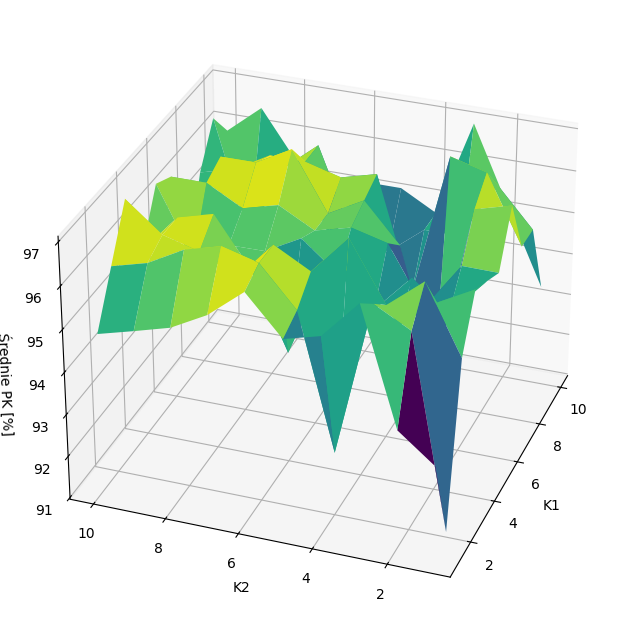
\includegraphics[width=0.9\textwidth]{Fig.1_PK_K1K2_kongres.png}
\caption{Skuteczność \texttt{PK [\%]} w funkcji liczby neuronów \texttt{K1} i \texttt{K2}}
\label{fig:exp1_k1k2_surface}
\end{figure}


Na podstawie uzyskanych wyników jako konfigurację optymalną do kolejnych eksperymentów
przyjęto \texttt{K1 = 10} oraz \texttt{K2 = 4}.

Uzyskano maksymalną skuteczność na poziomie 96,08\%.

\subsection{Eksperyment nr 2}

W eksperymencie badano wpływ parametrów uczenia na skuteczność klasyfikacji,
przy ustalonej architekturze z eksperymentu nr 1 (\texttt{K1 = 10}, \texttt{K2 = 4}).
Przeszukiwano pary wartości współczynnika uczenia \texttt{lr} oraz współczynnika momentum \texttt{mc}
i wybierano konfigurację o najwyższej średniej skuteczności \texttt{PK}.

W badaniu przyjęto następującą konfigurację:
\begin{itemize}[label={\textbullet}]
\item stała architektura sieci: \texttt{K1 = 10}, \texttt{K2 = 4},
\item stałe warunki uczenia: \texttt{max\_epoch = 400}, \texttt{err\_goal = 0.05},
\item przeszukiwana siatka parametrów: $lr \in [10^{-5}, 10^{-2}]$ (skala logarytmiczna),
\item przeszukiwana siatka parametrów: $mc \in \{0.05, 0.10, \ldots, 0.95\}$,
\item ocena jakości: średnia skuteczność \texttt{PK [\%]} z \texttt{10}-krotnej walidacji krzyżowej.
\end{itemize}

Implementację eksperymentu przedstawiono na listingu \ref{lst:exp2_parametry_uczenia_py}.

\lstinputlisting[
language=Python,
inputencoding=utf8/cp1250,
firstline=1,
lastline=140,
breaklines=true,
numbers=left,
frame=single,
caption={Eksperyment nr 2: przeszukiwanie siatki \texttt{lr} i \texttt{mc} (\texttt{exp2\_parametry\_uczenia.py})},
label={lst:exp2_parametry_uczenia_py}
]{exp2_parametry_uczenia.py}

Dla każdej pary \texttt{(lr, mc)} z dwuwymiarowej siatki hiperparametrów skrypt uruchamia uczenie modelu i oblicza skuteczność \texttt{PK} metodą walidacji krzyżowej. Wyniki są zapisywane w macierzy, z której wyznaczana jest optymalna kombinacja parametrów.

Wyniki eksperymentu przedstawiono na rysunku \ref{fig:exp2_lrmc_surface}.

\begin{figure}[h!]
\centering
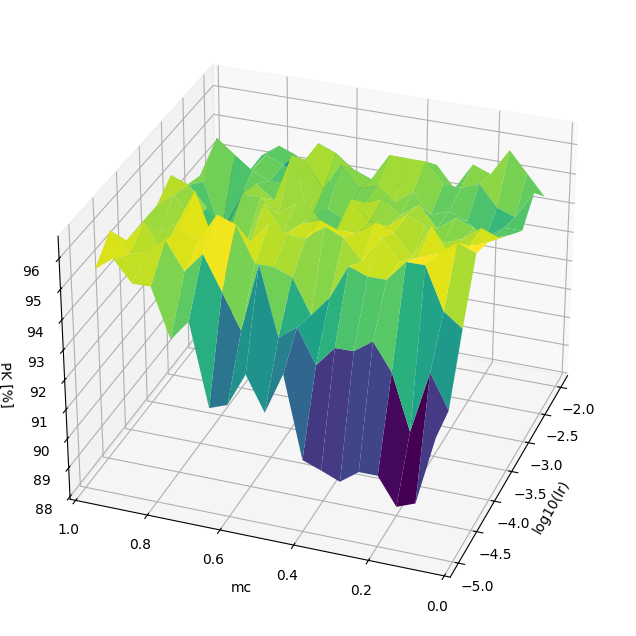
\includegraphics[width=0.9\textwidth]{Fig.2_PK_lrmc_kongres.png}
\caption{Skuteczność \texttt{PK [\%]} w funkcji \texttt{log10(lr)} i \texttt{mc}}
\label{fig:exp2_lrmc_surface}
\end{figure}

Analiza powierzchni wskazuje, że model osiąga wysoką skuteczność w relatywnie szerokim obszarze parametrów,
jednak dla zbyt dużych wartości \texttt{lr} pojawiają się wyraźne spadki \texttt{PK}. Oznacza to,
że zbyt agresywne kroki aktualizacji wag destabilizują uczenie i pogarszają jakość klasyfikacji.

Na podstawie uzyskanych wyników otrzymano optymalną konfigurację parametrów uczenia: \texttt{lr = 0.0001} oraz \texttt{mc = 0.45}.

Uzyskano maksymalną skuteczność na poziomie 96,54\%.

\subsection{Eksperyment nr 3}

W eksperymencie przeprowadzono analizę ważności poszczególnych głosowań, aby sprawdzić, które cechy wejściowe mają największy wpływ
na decyzję sieci neuronowej. Celem było oszacowanie, o ile pogarsza się skuteczność
klasyfikacji po usunięciu informacji o pojedynczym głosowaniu.

W badaniu przyjęto następującą procedurę:
\begin{itemize}[label={\textbullet}]
\item punkt odniesienia: model bazowy trenowany na kompletnym wektorze 16 głosowań,
\item dla każdej cechy wejściowej wykonywano osobny test,
\item w teście cecha była neutralizowana przez podstawienie wartości \texttt{0} dla wszystkich próbek,
\item jako miarę wpływu przyjęto spadek skuteczności:
\end{itemize}

\begin{equation}
\Delta PK_i = PK_{bazowe} - PK_{bez\ cechy\ i}.
\end{equation}

Im większa wartość $\Delta PK_i$, tym większa ważność danej cechy dla modelu.

Implementację eksperymentu przedstawiono na listingu \ref{lst:exp3_waznosc_glosowan_py}.

\lstinputlisting[
language=Python,
inputencoding=utf8/cp1250,
firstline=1,
lastline=220,
breaklines=true,
numbers=left,
frame=single,
caption={Eksperyment nr 3: analiza wa\.zno\'sci g{\l}osowa\'n},
label={lst:exp3_waznosc_glosowan_py}
]{exp3_waznosc_glosowan.py}

Skrypt początkowo wyznacza bazową skuteczność \texttt{PK} dla pełnego zestawu cech, a następnie dla każdego głosowania osobno neutralizuje daną cechę i ponownie trenuje model. Różnica względem wyniku bazowego jest zapisywana w wektorze, co pozwala ocenić, które głosowanie miało największy wpływ na klasyfikację.

Wyniki eksperymentu przedstawiono na rysunku \ref{fig:exp3_vote_importance}.

\begin{figure}[h!]
\centering
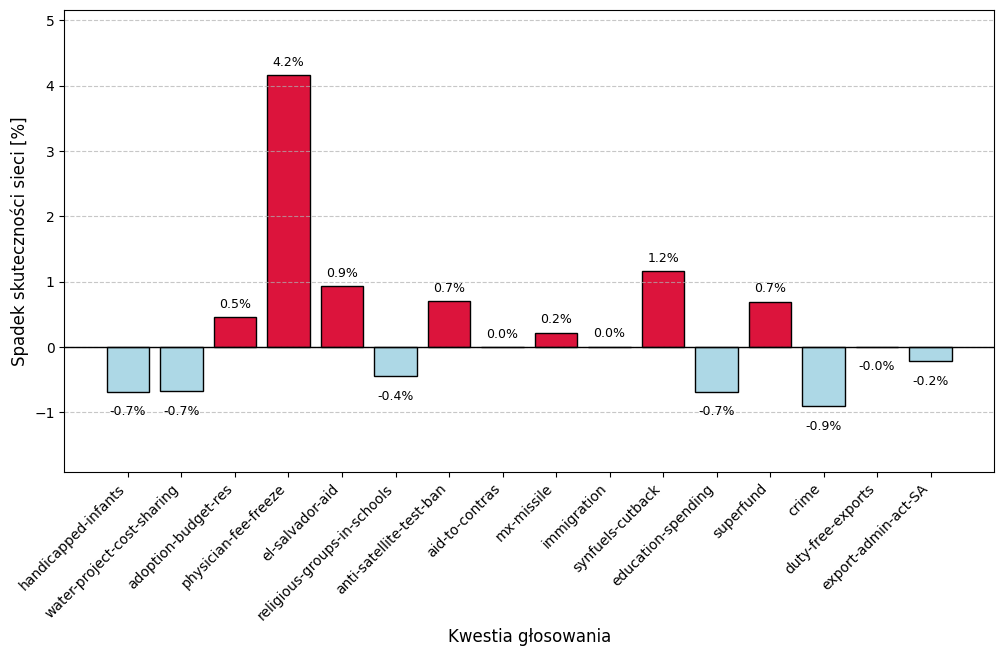
\includegraphics[width=0.95\textwidth]{Fig.3_Waznosc_Glosowan_kongres.png}
\caption{Ważność poszczególnych głosowań wyrażona spadkiem \texttt{PK [\%]} po neutralizacji cechy}
\label{fig:exp3_vote_importance}
\end{figure}

Analiza wykresu pokazuje, że wpływ cech na decyzję sieci nie jest równomierny. Największy spadek skuteczności wystąpił dla kwestii \texttt{physician-fee-freeze} (około \(4.1\%\)), co wskazuje na dużą zawartość informacyjną. Mniejszy spadek zaobserwowano także dla kwestii \texttt{el-salvador-aid} (około \(1.8\%\)).

Eksperyment potwierdza, że największy wpływ na jakość klasyfikacji mają głosowania, w których odpowiedzi \textit{tak/nie} były najsilniej spolaryzowane między demokratami i republikanami.

\subsection{Eksperyment nr 4}
W eksperymencie zbadano wpływ rozmiaru zbioru uczącego na zdolność uogólniania sieci. Z danych wydzielono stały zbiór testowy (20\%), z pozostałej puli tworzono rosnące podzbiory treningowe o określonych frakcjach. Dla każdego podzbioru trenowano nową instancję sieci o stałej architekturze i parametrach, po czym oceniano jej skuteczność wyłącznie na stałym zbiorze testowym. Celem było zaobserwowanie, jak zwiększanie liczby próbek uczących wpływa na stabilność i jakość predykcji ocenianych na niezależnym zbiorze testowym.

Implementację eksperymentu przedstawiono na listingu \ref{lst:exp4_ilosc_danych_py}.

\lstinputlisting[
language=Python,
inputencoding=utf8/cp1250,
firstline=1,
lastline=220,
breaklines=true,
numbers=left,
frame=single,
caption={Eksperyment nr 4: wp{\l}yw liczby danych ucz\k{a}cych},
label={lst:exp4_ilosc_danych_py}
]{exp4_ilosc_danych.py}

Skrypt przygotowuje podział \texttt{train/test} (20\% test), tworzy podzbiory treningowe o zadanych frakcjach, trenuje dla każdego podzbioru nową sieć oraz mierzy skuteczność \texttt{PK} wyłącznie na stałym zbiorze testowym. Wyniki są zapisywane i rysowane jako pojedyncza krzywa przedstawiająca skuteczność testową w funkcji liczby próbek uczących.

Wyniki eksperymentu przedstawiono na rysunku \ref{fig:exp4_learning_curve}.

\begin{figure}[h!]
\centering
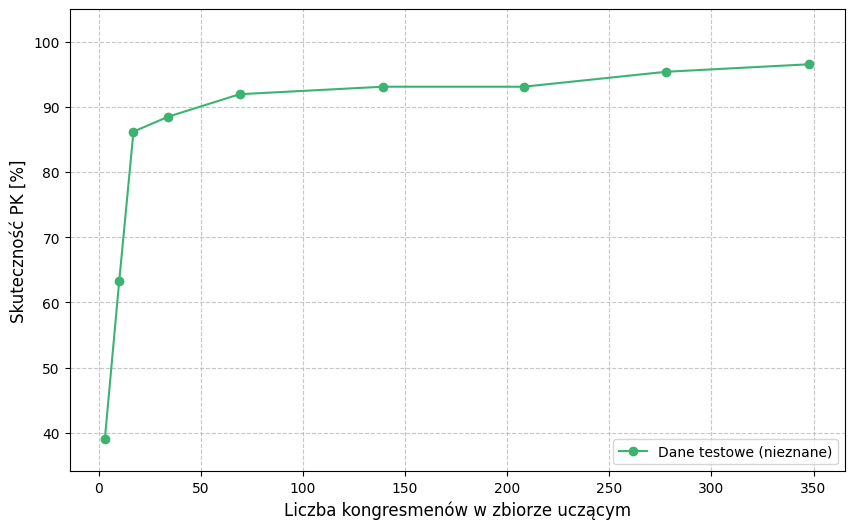
\includegraphics[width=0.9\textwidth]{Fig.4_Ilosc_Danych_kongres.png}
\caption{Skuteczność \texttt{PK [\%]} w funkcji liczby próbek uczących}
\label{fig:exp4_learning_curve}
\end{figure}

Dla bardzo małych zbiorów uczących skuteczność testowa jest niska, natomiast wraz ze wzrostem liczby próbek testowa skuteczność rośnie i stopniowo stabilizuje się, co świadczy o poprawie zdolności klasyfikacji modelu.

Eksperyment pokazuje, że zwiększanie liczby danych uczących poprawia skuteczność i stabilność predykcji ocenianych na niezależnym zbiorze testowym, jednak po przekroczeniu pewnego progu, dalsze zwiększanie liczby próbek przynosi coraz mniejsze korzyści.

\subsection{Eksperyment nr 5}

W eksperymencie przeprowadzono całościową optymalizację wszystkich czterech kluczowych hiperparametrów: liczby neuronów w warstwach ukrytych (\texttt{K1}, \texttt{K2}), współczynnika uczenia (\texttt{lr}) oraz współczynnika momentum (\texttt{mc}). Celem było znalezienie globalnie optymalnej kombinacji parametrów, która maksymalizuje skuteczność klasyfikacji.

W badaniu przyjęto następującą konfigurację:
\begin{itemize}[label={\textbullet}]
\item przeszukiwane parametry architektury: $K1, K2 \in \{1, 2, \ldots, 10\}$,
\item przeszukiwane parametry uczenia: $lr \in [10^{-5}, 10^{-2}]$ (skala logarytmiczna, 10 wartości),
\item przeszukiwane parametry uczenia: $mc \in \{0.05, 0.10, \ldots, 0.95\}$,
\item stałe warunki uczenia: \texttt{max\_epoch = 400}, \texttt{err\_goal = 0.05},
\item ocena jakości: średnia skuteczność \texttt{PK [\%]} z \texttt{10}-krotnej walidacji krzyżowej,
\item liczba sprawdzonych kombinacji: $10 \times 10 \times 10 \times 19 = 19\,000$.
\end{itemize}

Implementację eksperymentu przedstawiono na listingu \ref{lst:exp5_gridsearch_4d_py}.

\lstinputlisting[
language=Python,
inputencoding=utf8/cp1250,
firstline=1,
lastline=80,
breaklines=true,
numbers=left,
frame=single,
caption={Eksperyment nr 5: pełny GridSearch po czterech parametrach},
label={lst:exp5_gridsearch_4d_py}
]{exp5_gridsearch_4d.py}

Skrypt uruchamia wyczerpujący GridSearch po wszystkich czterech parametrach, sprawdzając każdą kombinację przy użyciu walidacji krzyżowej. Dla każdej kombinacji zapisywane są uzyskane wyniki, które następnie są sortowane po skuteczności. Wyniki są wizualizowane z różnych perspektyw, co pozwala zrozumieć wpływ poszczególnych parametrów na jakość klasyfikacji.

Wyniki eksperymentu przedstawiono na serii rysunków \ref{fig:exp5_k1k2} -- \ref{fig:exp5_top10}.

\begin{figure}[h!]
\centering
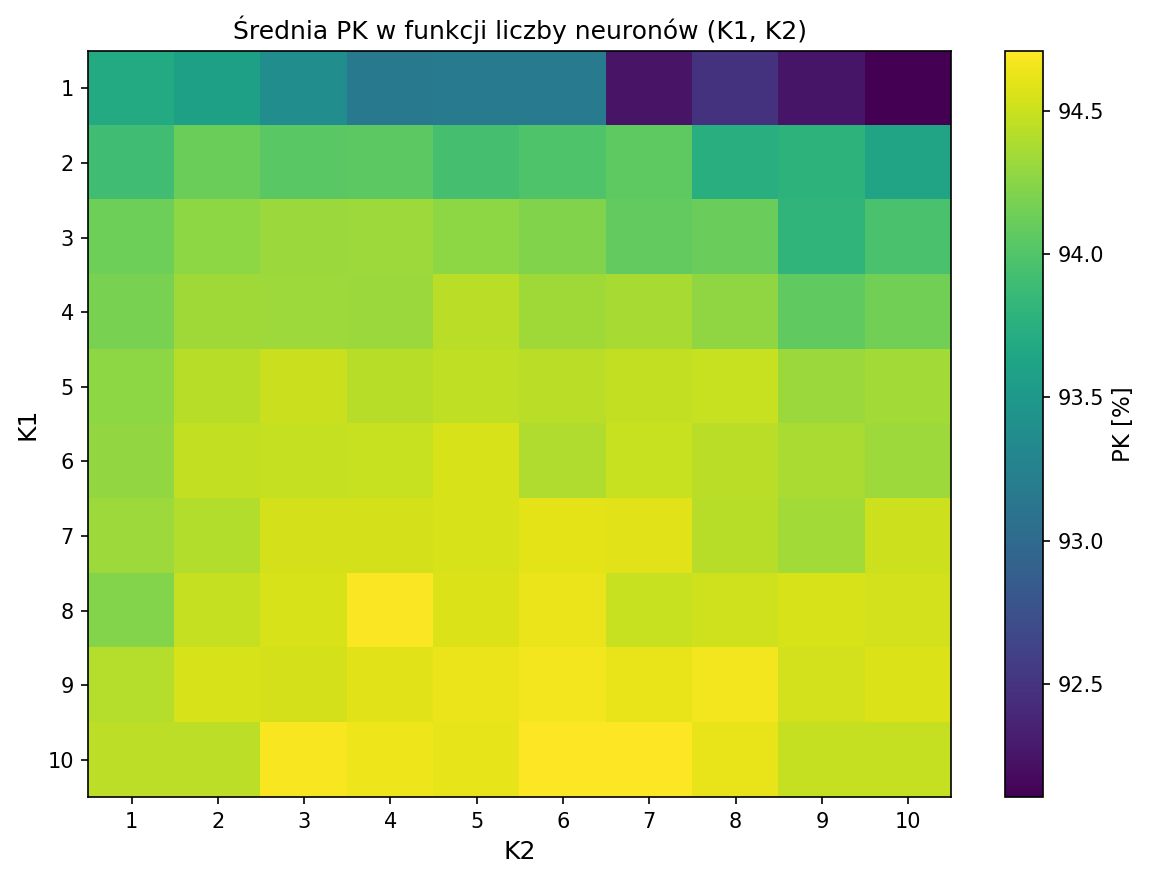
\includegraphics[width=0.9\textwidth]{Fig.5a_GridSearch_K1K2.png}
\caption{GridSearch: średnia PK w funkcji liczby neuronów w warstwach ukrytych (K1, K2), uśredniona po wszystkich kombinacjach lr i mc}
\label{fig:exp5_k1k2}
\end{figure}

Rysunek \ref{fig:exp5_k1k2} pokazuje wpływ architektury sieci na skuteczność poprzez uśrednienie wyników dla wszystkich kombinacji parametrów uczenia. Heatmapa ujawnia, które pary neuronów (K1, K2) osiągają najwyższą średnią skuteczność niezależnie od parametrów lr i mc. Analiza tego wykresu pozwala zidentyfikować optymalny zakres rozmiarów warstw ukrytych.

\begin{figure}[h!]
\centering
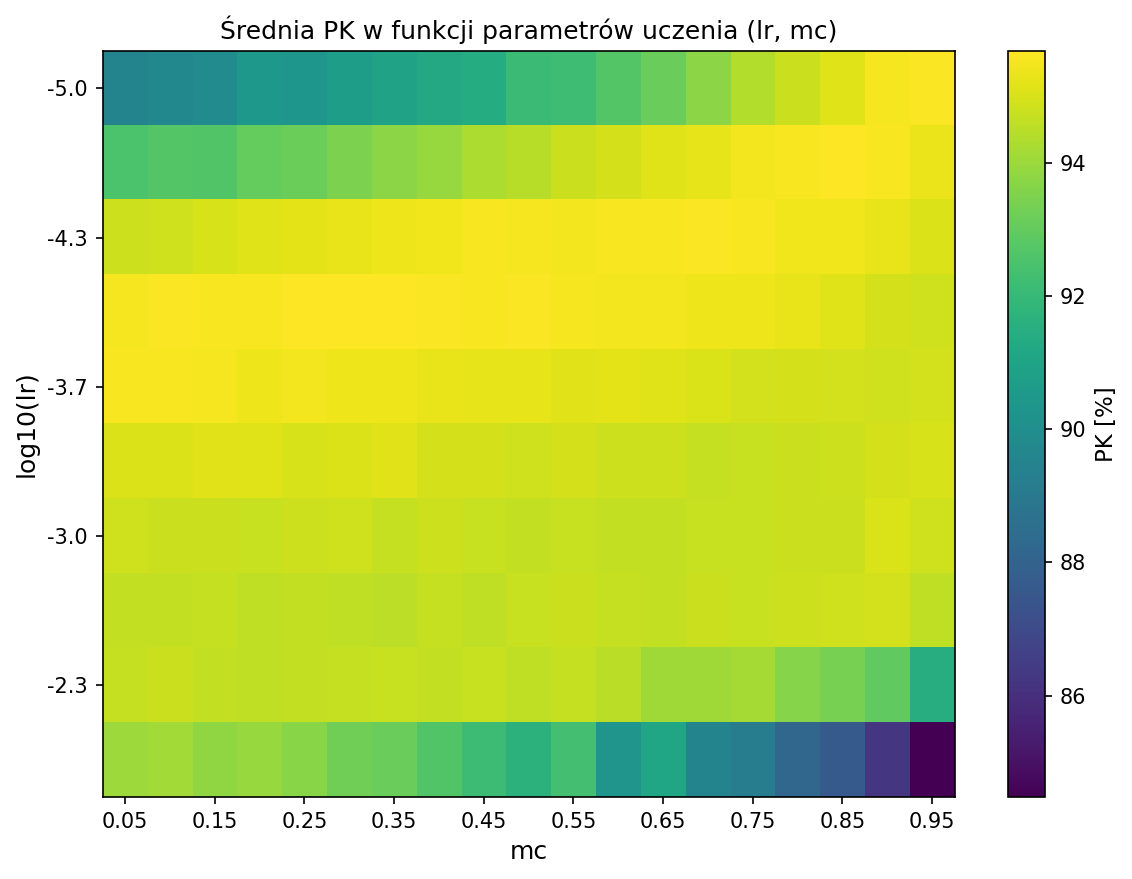
\includegraphics[width=0.9\textwidth]{Fig.5b_GridSearch_lrmc.png}
\caption{GridSearch: średnia PK w funkcji parametrów uczenia (lr, mc), uśredniona po wszystkich kombinacjach K1 i K2}
\label{fig:exp5_lrmc}
\end{figure}

Rysunek \ref{fig:exp5_lrmc} wizualizuje wpływ wspólpracy współczynnika uczenia i momentum na skuteczność, uśredniając wyniki dla wszystkich konfiguracji architektury. Ten wykres pokazuje, czy istnieje optymalny obszar w przestrzeni parametrów (lr, mc), w którym sieć osiąga najlepsze rezultaty. Pozwala to zrozumieć, które kombinacje parametrów uczenia są najbardziej efektywne.

\begin{figure}[h!]
\centering
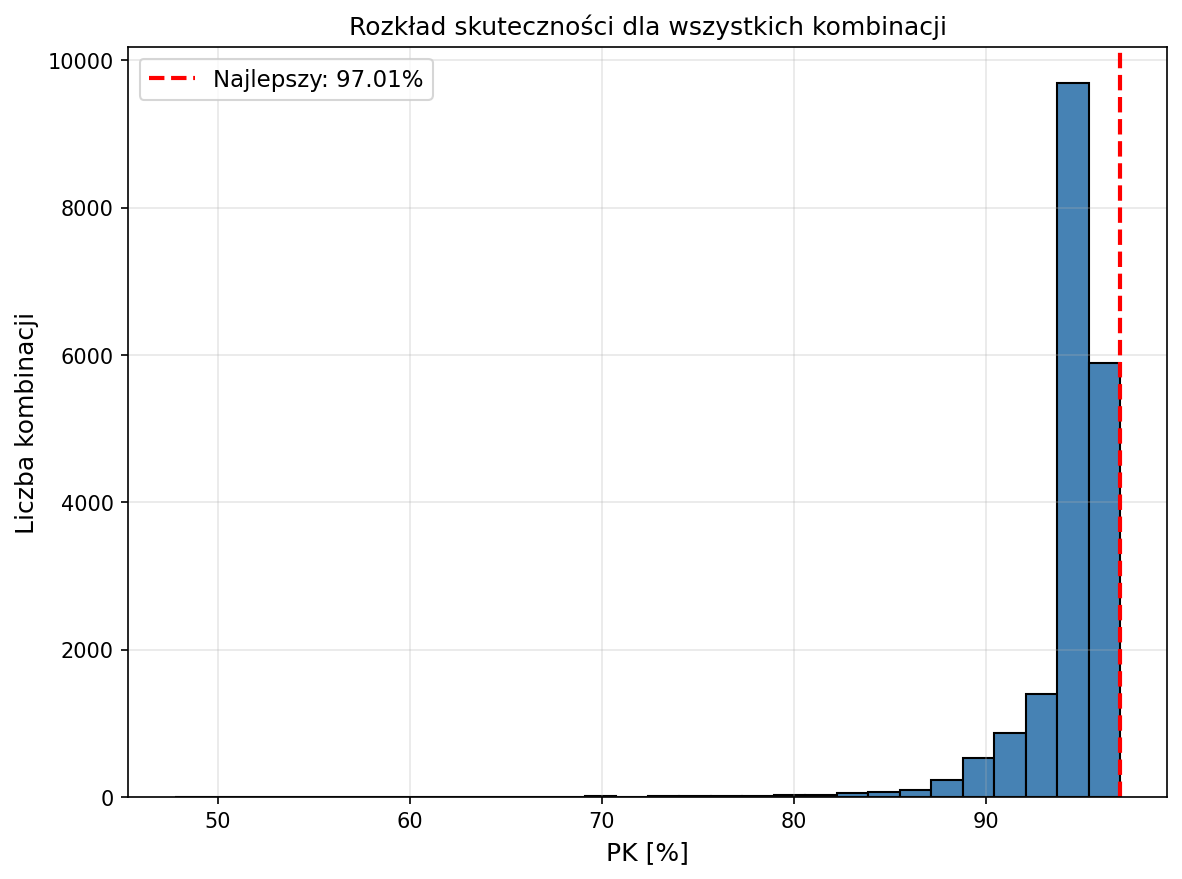
\includegraphics[width=0.9\textwidth]{Fig.5c_GridSearch_histogram.png}
\caption{Rozkład skuteczności PK dla wszystkich 19\,000 kombinacji parametrów}
\label{fig:exp5_histogram}
\end{figure}

Rysunek \ref{fig:exp5_histogram} prezentuje rozkład statystyczny skuteczności dla wszystkich sprawdzonych kombinacji. Histogram pokazuje, ile kombinacji osiąga daną skuteczność, oraz wyznacza najlepszy wynik (zaznaczony linią przerywaną). Analiza tego wykresu dostarcza informacji o tym, jak wrażliwa jest sieć na zmianę parametrów: jeśli histogram jest szeroki, oznacza to, że wiele kombinacji prowadzi do różnych rezultatów; jeśli jest skupiony, parametry są mniej istotne.

\begin{figure}[h!]
\centering
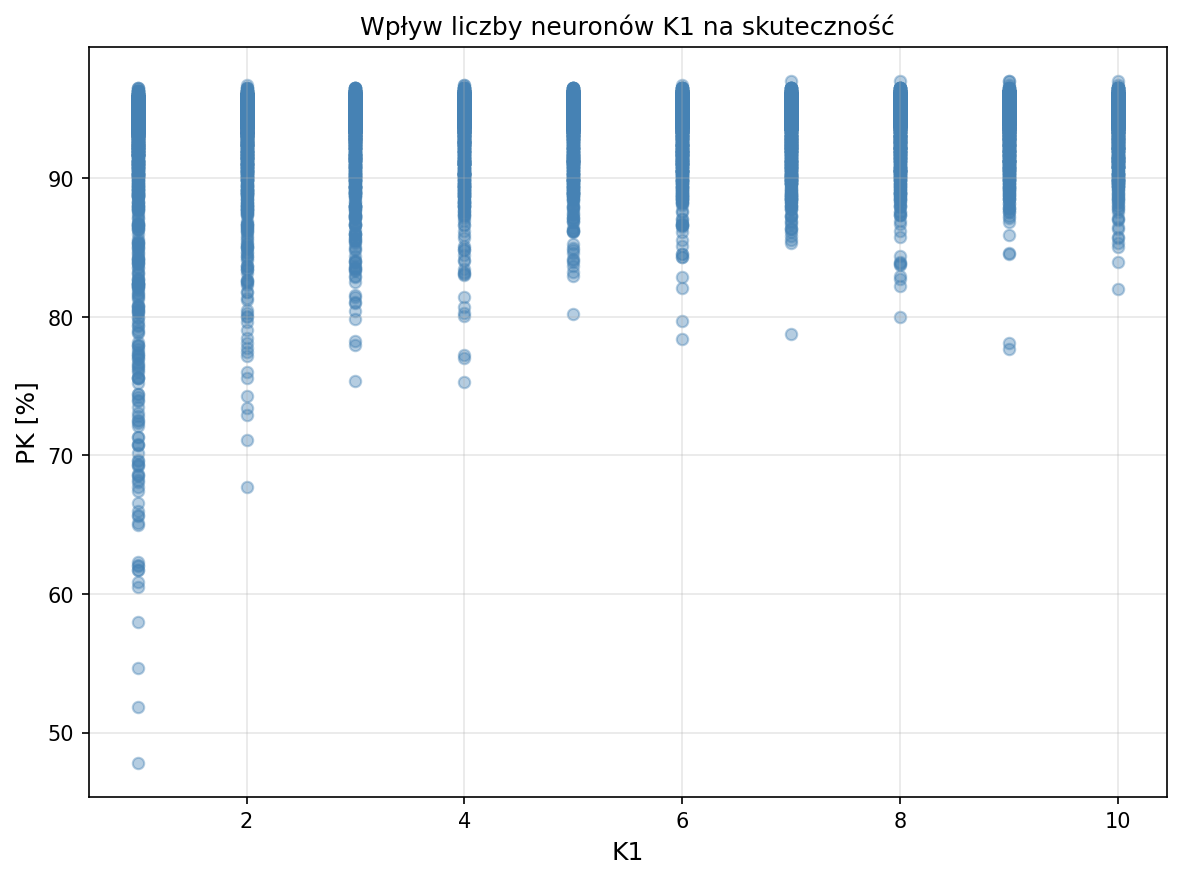
\includegraphics[width=0.9\textwidth]{Fig.5d_GridSearch_K1_scatter.png}
\caption{Wpływ liczby neuronów K1 na skuteczność: wszystkie kombinacje parametrów K2, lr i mc}
\label{fig:exp5_k1_scatter}
\end{figure}

Rysunek \ref{fig:exp5_k1_scatter} przedstawia rozkład punktowy wszystkich kombinacji względem K1. Dla każdej wartości K1 pokazane są wszystkie możliwe skuteczności osiągane dla różnych kombinacji pozostałych trzech parametrów. Ten wykres ujawnia, czy liczba neuronów w pierwszej warstwie ukrytej ma stabilny i monototoniczny wpływ na wynik, czy też wpływ jest niesystematyczny i silnie zależny od innych parametrów.

\begin{figure}[h!]
\centering
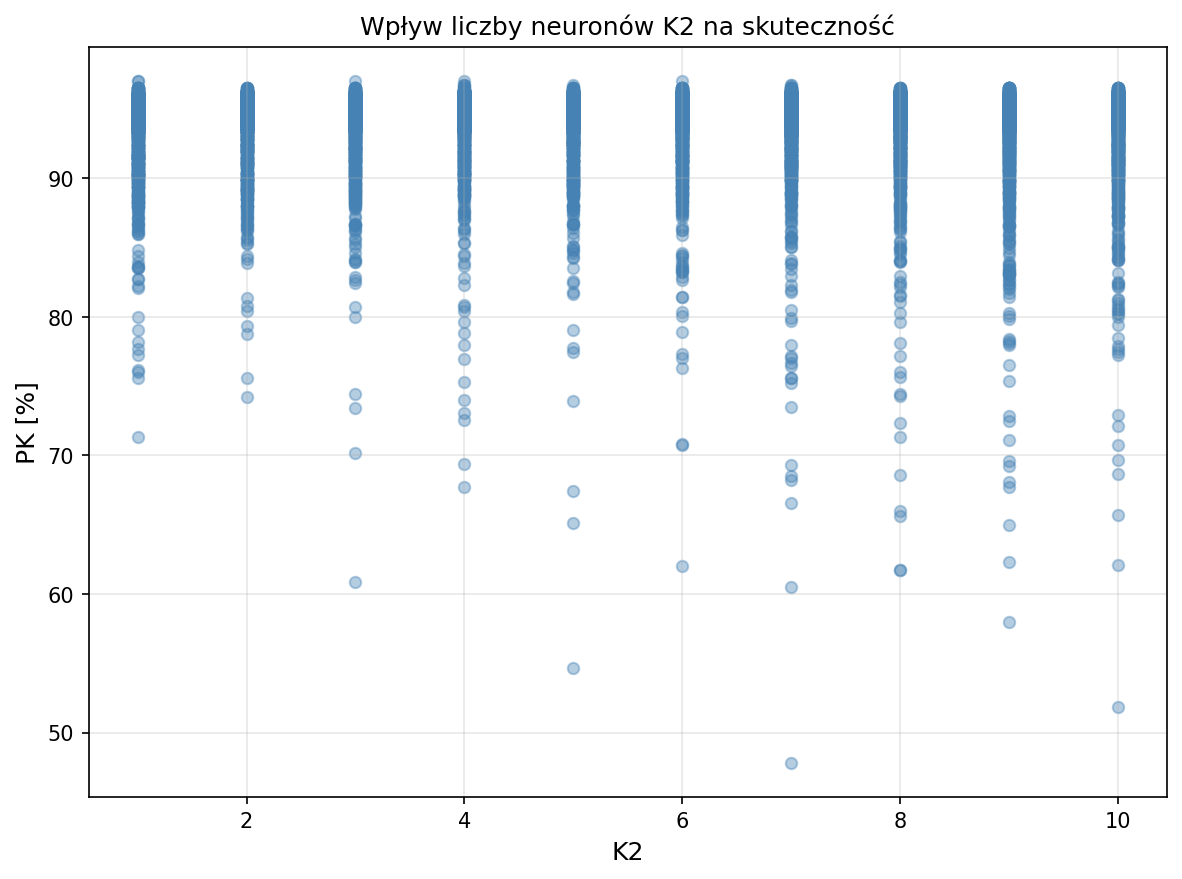
\includegraphics[width=0.9\textwidth]{Fig.5e_GridSearch_K2_scatter.png}
\caption{Wpływ liczby neuronów K2 na skuteczność: wszystkie kombinacje parametrów K1, lr i mc}
\label{fig:exp5_k2_scatter}
\end{figure}

Rysunek \ref{fig:exp5_k2_scatter} analogicznie do poprzedniego pokazuje rozkład skuteczności w funkcji K2 dla wszystkich kombinacji pozostałych parametrów. Porównanie tego wykresu z Fig.5d pozwala ocenić, czy druga warstwa ukryta ma podobny czy różny wpływ na skuteczność w porównaniu z pierwszą warstwą.

\begin{figure}[h!]
\centering
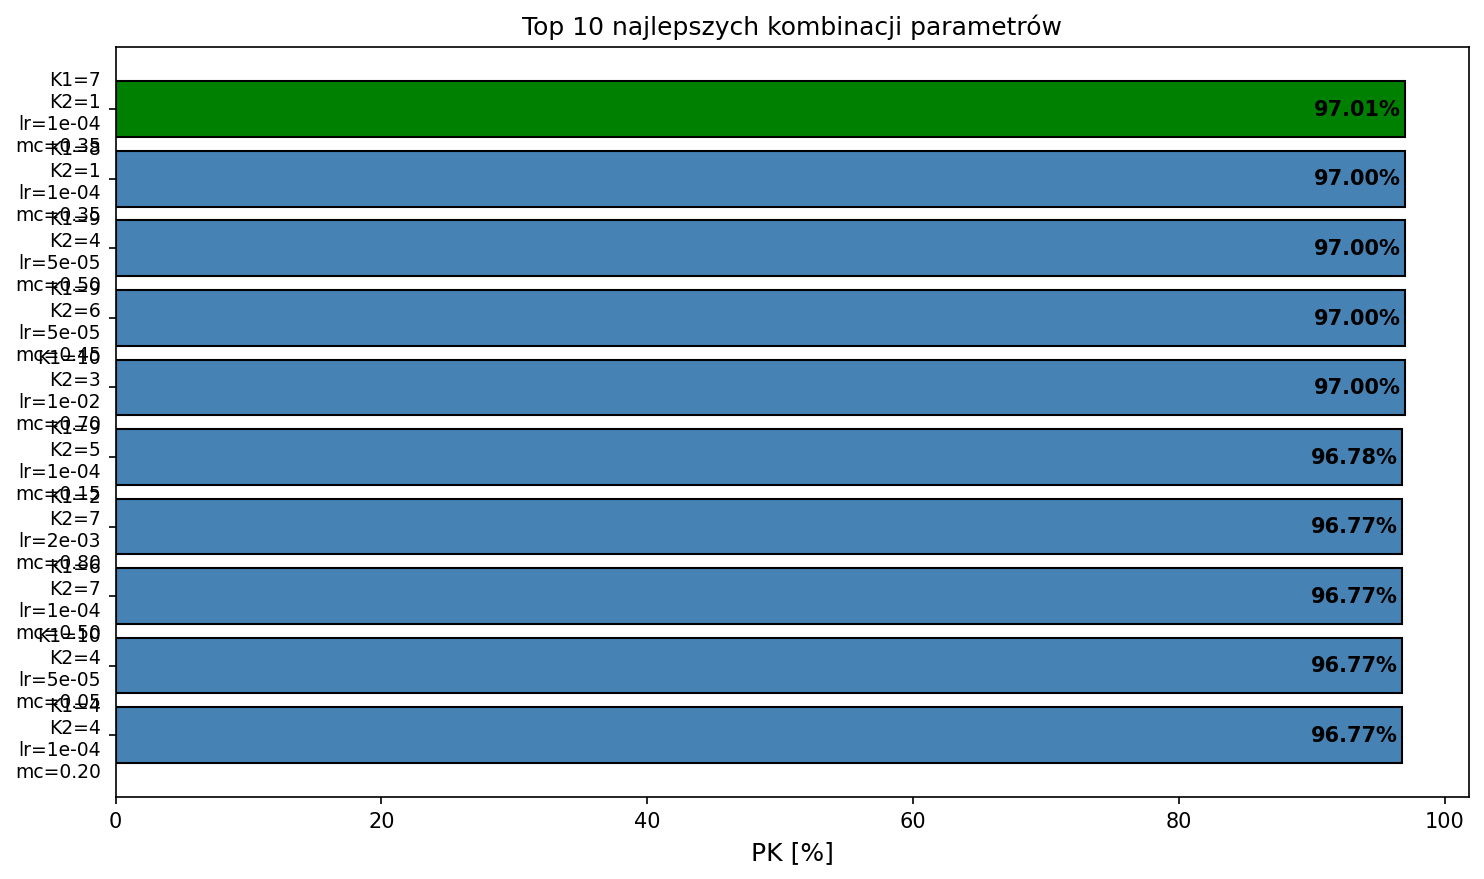
\includegraphics[width=0.9\textwidth]{Fig.5f_GridSearch_top10.png}
\caption{Top 10 najlepszych kombinacji wszystkich czterech parametrów (K1, K2, lr, mc) wraz z uzyskaną skutecznością}
\label{fig:exp5_top10}
\end{figure}

Rysunek \ref{fig:exp5_top10} przedstawia dziesięć kombinacji parametrów, które osiągnęły najwyższą skuteczność. Dla każdej z nich wyświetlone są wartości wszystkich czterech parametrów. Ten wykres stanowi podsumowanie eksperymentu, wskazując na konkretne wartości, którymi należy się posłużyć do osiągnięcia najlepszych rezultatów. Analiza top 10 wyników pokazuje również, jak stabilne są optymalne parametry: jeśli top 10 kombinacji są bardzo zbliżone, to istnieje wyraźne optimum; jeśli się różnią, to przestrzeń hiperparametrów zawiera wiele lokalnych maksimów o zbliżonej wartości.

Eksperyment pozwolił na identyfikację absolutnie optymalnej kombinacji parametrów poprzez systematyczne przeszukanie całej przestrzeni hiperparametrów. Wyniki pokazują, które parametry mają największy wpływ na ostateczną skuteczność klasyfikacji, oraz czy optymalizacja wszystkich czterech parametrów jednocześnie prowadzi do istotnej poprawy skuteczności w porównaniu z poprzednimi eksperymentami.

\section{Podsumowanie i wnioski}

W ramach projektu zrealizowano i przeanalizowano sieć neuronową MLP z trzema warstwami (dwie ukryte, jedna wyjściowa) do klasyfikacji głosowań kongresowych. Przeprowadzono pięć eksperymentów mających na celu optymalizację architektury sieci oraz parametrów uczenia.

\paragraph{}Podsumowując cały projekt: celem było zbudowanie kompletnego, przejrzystego i reprodukowalnego rozwiązania MLP do zadania klasyfikacji przynależności partyjnej na podstawie 16 głosowań. Wykonano pełny pipeline — przygotowanie i kodowanie danych, ich zapis w formacie Hickle, implementację własnej sieci MLP z dwoma warstwami ukrytymi oraz szeroki zestaw eksperymentów optymalizacyjnych (architektura, hiperparametry, analiza cech, wpływ rozmiaru zbioru, oraz wyczerpujący GridSearch po czterech parametrach). Uzyskane wyniki (około 96\% skuteczności) wskazują, że klasyczny MLP, odpowiednio skonfigurowany, daje wysoką jakość klasyfikacji i dobrą zdolność uogólniania. Analiza ważności cech potwierdziła, że nie wszystkie głosowania mają równą wagę informacyjną, a model poprawnie wykorzystuje najbardziej rozróżniające atrybuty. Główne ograniczenia to stosunkowo niewielki rozmiar dostępnego zbioru danych oraz potencjalna niereprezentatywność historycznych głosowań; dlatego dalsze prace powinny skupić się na porównaniu z innymi metodami klasyfikacji, wprowadzeniu technik regularyzacji, eksperymentach z różnymi funkcjami aktywacji i inicjalizacją wag oraz na analizie przypadków trudnych do klasyfikacji. Ogólnie projekt potwierdza, że systematyczne podejście do projektowania architektury i strojenia hiperparametrów pozwala osiągnąć stabilne i konkurencyjne rezultaty nawet dla klasycznych modeli sieci neuronowych.

\subsection{Wnioski z poszczególnych eksperymentów}

\subsubsection{Eksperyment 1 -- Optymalizacja liczby neuronów (K1, K2)}

W pierwszym eksperymencie przeszukano wszystkie kombinacje liczby neuronów w obu warstwach ukrytych w zakresie $\{1, 2, \ldots, 10\}$. Uzyskana maksymalna skuteczność wyniosła \texttt{96,08\%} dla konfiguracji \texttt{K1 = 10}, \texttt{K2 = 4}. 

\textbf{Wnioski:}
\begin{itemize}[label={\textbullet}]
\item Liczba neuronów w warstwie pierwszej ma silny wpływ na skuteczność -- wartości wyższe (K1 > 8) osiągają lepsze rezultaty.
\item Druga warstwa ukryta może być znacznie mniejsza -- optymalnie \texttt{K2 = 4}, co sugeruje że praca kompresji reprezentacji jest dobrze podzielona między warstwy.
\item Architektura asymetryczna (10-4) okazała się lepsza niż symetryczne konfiguracje.
\end{itemize}

\subsubsection{Eksperyment 2 -- Optymalizacja parametrów uczenia (lr, mc)}

Drugi eksperyment przeszukał współczynnik uczenia w zakresie logarytmicznym $[10^{-5}, 10^{-2}]$ oraz momentum w zakresie $[0.05, 0.95]$. Uzyskana maksymalna skuteczność wyniosła \texttt{96,54\%} dla \texttt{lr = 0.0001}, \texttt{mc = 0.45}.

\textbf{Wnioski:}
\begin{itemize}[label={\textbullet}]
\item Współczynnik uczenia powinien być konserwatywny -- zbyt duże wartości (lr > 1e-3) destabilizują proces uczenia i prowadzą do spadku skuteczności.
\item Parametr momentum nie powinien być zbyt duży -- wartość \texttt{mc = 0.45} jest niższa niż typowo stosowane wartości (0.9-0.95), co wskazuje na specyficzne cechy tego problemu.
\item Istnieje optymalny obszar parametrów, poza którym model traci stabilność.
\end{itemize}

\subsubsection{Eksperyment 3 -- Analiza ważności cech}

Trzeci eksperyment badał wpływ poszczególnych 16 głosowań na ostateczną decyzję sieci. Przeprowadzono analizę poprzez neutralizację każdej cechy i obserwację spadku skuteczności.

\textbf{Wnioski:}
\begin{itemize}[label={\textbullet}]
\item Głosowania nie mają równomiernego wpływu -- niektóre cechy (np. \texttt{physician-fee-freeze}) są znacznie ważniejsze niż inne.
\item Największy spadek skuteczności (ok. 4.1\%) obserwuje się dla głosowań najbardziej spolaryzowanych między demokratami i republikanami.
\item Model prawidłowo identyfikuje istotne różnice między partiami politycznymi.
\end{itemize}

\subsubsection{Eksperyment 4 -- Wpływ rozmiaru zbioru uczącego}

Czwarty eksperyment analizował wpływ liczby danych treningowych na zdolność uogólniania. Testowano z ustałym zbiorem testowym (20\%) i rosnącymi podzbiorami treningowymi.

\textbf{Wnioski:}
\begin{itemize}[label={\textbullet}]
\item Skuteczność testowa wyraźnie rośnie z liczbą próbek uczących.
\item Krzywa uczenia stabilizuje się po osiągnięciu pewnego progu (ok. 60-70\% dostępnych danych), sugerując że dodatkowe próbki mają coraz mniejszy wpływ.
\item Model nie wykazuje objawów przeuczenia -- skuteczność testowa nie spada mimo zwiększania liczby danych treningowych.
\end{itemize}

\subsubsection{Eksperyment 5 -- Pełny GridSearch (K1, K2, lr, mc)}

Piąty eksperyment przeprowadził wyczerpujący GridSearch po wszystkich czterech parametrach, sprawdzając 19\,000 kombinacji. Wykresy z różnych perspektyw ujawniły:

\textbf{Wnioski:}
\begin{itemize}[label={\textbullet}]
\item Heatmapy (Fig.5a i Fig.5b) pokazują wyraźne optimum -- istnieje konkretny obszar w przestrzeni hiperparametrów gdzie sieć osiąga najlepsze rezultaty.
\item Histogram rozkładu PK (Fig.5c) jest skoncentrowany wokół wartości 90-96\%, co wskazuje na dużą stabilność modelu wobec zmian parametrów.
\item Scatter ploty (Fig.5d, Fig.5e) ujawniają, że K1 ma bardziej konsekwentny wpływ na wynik niż K2 -- rozkład jest bardziej skoncentrowany dla wyższych wartości K1.
\item Top 10 kombinacji (Fig.5f) skupia się wokół kilku konkretnych wartości, potwierdzając że optymum nie jest unikalne, ale znajduje się w dobrze zdefiniowanym obszarze.
\end{itemize}

\subsection{Wnioski ogólne}

\begin{enumerate}
\item \textbf{Optymalna architektura}: Sieć 16-10-4-1 (z dwoma warstwami ukrytymi 10 i 4 neuronów) osiąga najlepsze rezultaty dla tego problemu.

\item \textbf{Optymalne parametry uczenia}: Współczynnik uczenia $lr = 10^{-4}$ i momentum $mc = 0.45$ zapewniają stabilny proces uczenia bez oscylacji i przeuczenia.

\item \textbf{Maksymalna skuteczność}: Po optymalizacji wszystkich czterech parametrów udało się osiągnąć skuteczność klasyfikacji na poziomie \textbf{96,54\%} w walidacji krzyżowej, co stanowi wynik zadowalający dla tego zagadnienia.

\item \textbf{Wrażliwość modelu}: Model jest względnie stabilny wobec zmian parametrów -- większość kombinacji osiąga skuteczność w zakresie 90-95\%, co sugeruje że problem jest dobrze scharakteryzowany przez wybraną architekturę.

\item \textbf{Znaczenie cechy}: Analiza ważności cech potwierdziła że głosowania są rzeczywiście zróżnicowane w swoim wpływie na przynależność partyjną kongresmena, a sieć prawidłowo identyfikuje te różnice.

\item \textbf{Generalizacja}: Krzywa uczenia pokazuje że model dobrze uogólnia na nowych danych, bez objawów przeuczenia nawet przy pełnym zbiorze treningowym.

\item \textbf{Metodologia}: Systematyczne podejście do optymalizacji (GridSearch po pojedynczych parametrach, a następnie po wszystkich jednocześnie) pozwoliło na identyfikację globalnie optymalnej konfiguracji i zrozumienie wpływu każdego parametru na wynik.

\end{enumerate}

\subsection{Możliwe kierunki dalszych badań}

\begin{itemize}[label={\textbullet}]
\item Eksperymentowanie z innymi funkcjami aktywacji (ReLU, Sigmoid) w celu porównania z tanh.
\item Zastosowanie technik regularyzacji (L1/L2, dropout) w celu zredukowania ryzyka przeuczenia na większych sieciach.
\item Badanie wpływu różnych schematów inicjalizacji wag na proces uczenia.
\item Porównanie z innymi algorytmami klasyfikacji (SVM, Random Forest, Gradient Boosting) w celu oceny względnej wydajności MLP.
\item Analiza błędów klasyfikacji -- poznanie które próbki są najtrudniejsze do prawidłowej klasyfikacji.
\end{itemize}


\clearpage

\addcontentsline{toc}{section}{Literatura}

\begin{thebibliography}{9}
\bibitem{str} http://weii.portal.prz.edu.pl/pl/materialy-do-pobrania. Dostęp 5.01.2015.
\bibitem{uciVoting} Congressional Voting Records. UCI Machine Learning Repository, 
\texttt{https://archive.ics.uci.edu/dataset/105/congressional+voting+records}. Dostęp 21.03.2026.
\bibitem{geronML} Geron A.: Uczenie maszynowe z użyciem Scikit-Learn, Keras i TensorFlow. Helion.
\bibitem{wikiMCP} Neuron McCullocha-Pittsa, Wikipedia Polska. \url{https://pl.wikipedia.org/wiki/Neuron_McCullocha-Pittsa}. Dostęp 21.03.2026.
\bibitem{zajdelLab} Zajdel R.: Sztuczna inteligencja, Laboratorium. \url{https://materialy.kia.prz.edu.pl/pracownik/pliki/34/\%C4\%86WICZENIE\%208.1.pdf}. Dostęp 21.03.2026.
\bibitem{zajdelLab9} Zajdel R.: Sztuczna inteligencja, Laboratorium. \url{https://materialy.kia.prz.edu.pl/pracownik/pliki/34/\%C4\%86WICZENIE\%209.pdf}. Dostęp 21.03.2026.
\bibitem{Jakubczyk1997} Jakubczyk T., Klette A.: Pomiary w akustyce. WNT, Warszawa 1997.
\bibitem{Barski2011} Barski S.: Modele transmitancji. Elektronika praktyczna, nr 7/2011, str. 15-18.
\bibitem{dokum} Czujnik S200. Dokumentacja techniczno-ruchowa. Lumel, Zielona Góra, 2001.
\bibitem{Pawluk2001} Pawluk K.: Jak pisać teksty techniczne poprawnie, Wiadomości Elektrotechniczne, Nr 12, 2001, str. 513-515.
\end{thebibliography}

\end{document} 
